\chapter{PJ3}


\section{記分板}




	
\begin{figure}
  \centering
  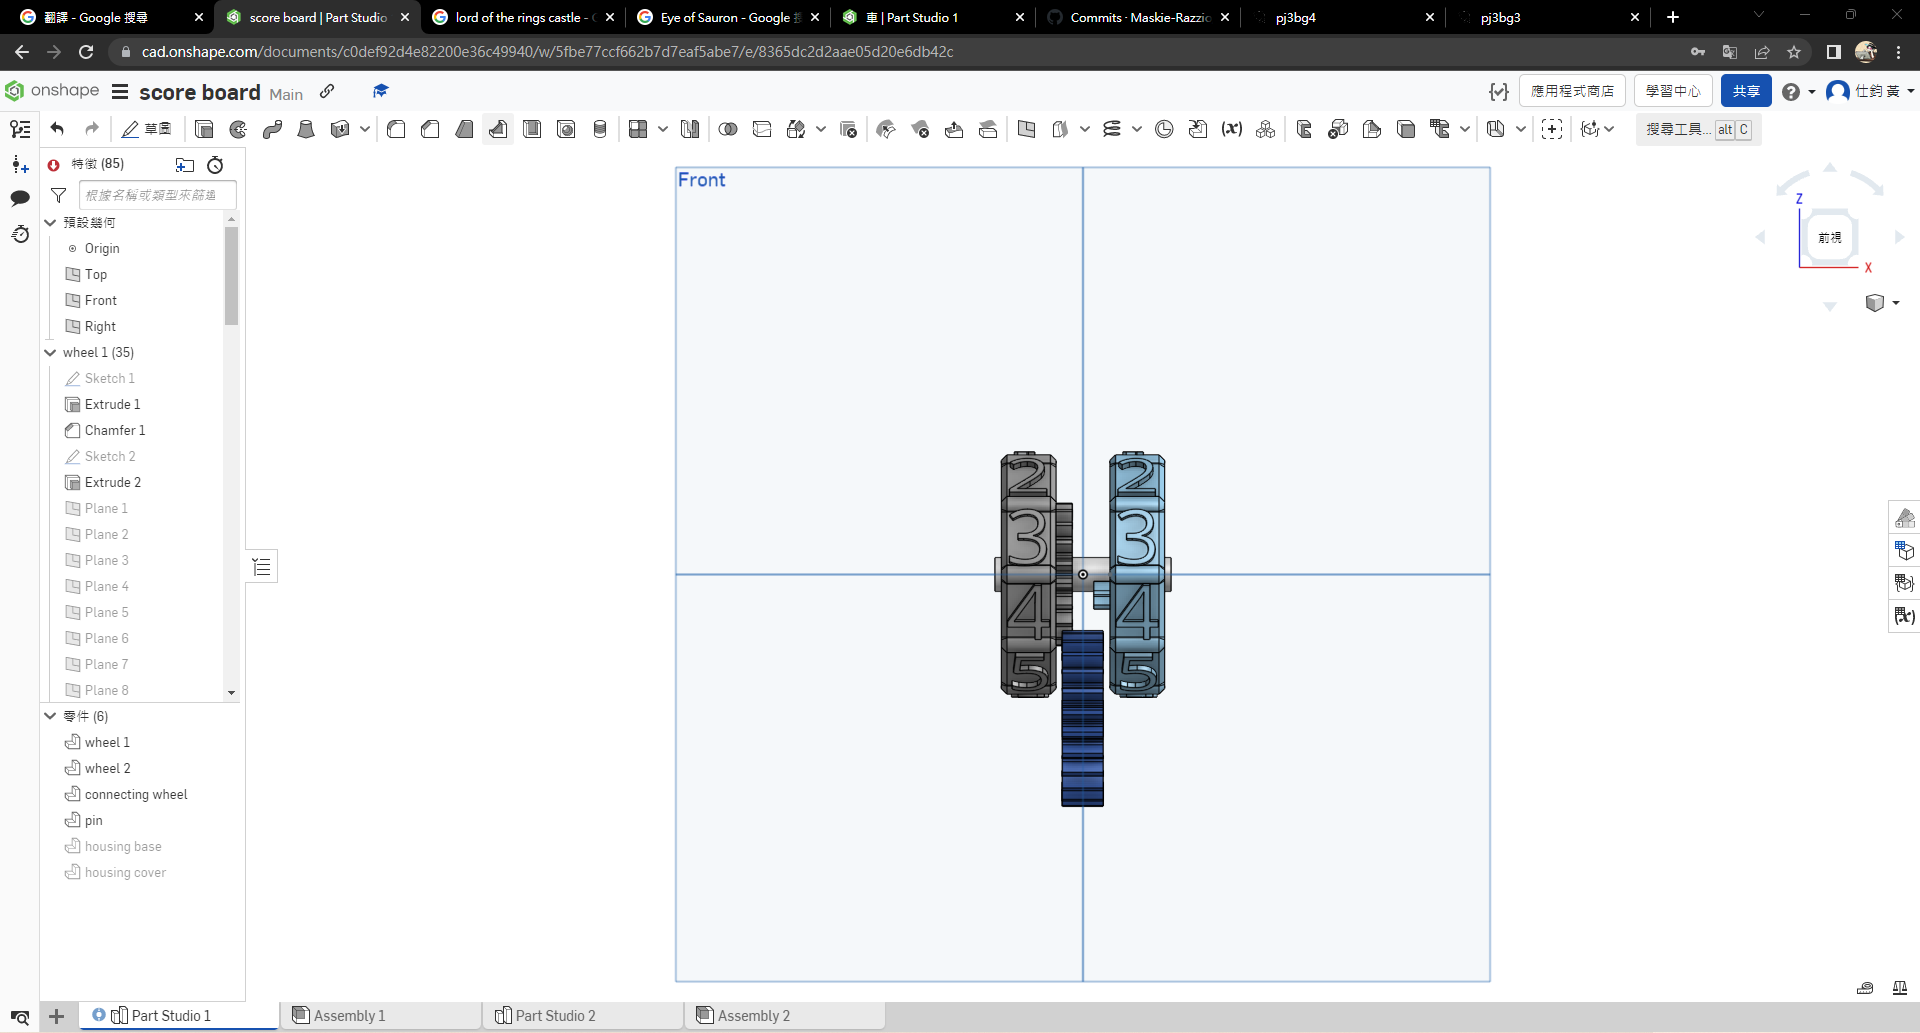
\includegraphics[width=0.5\textwidth]{timer1.png}
  \caption{次代記分板設計圖1}
  
\end{figure}

\begin{figure}
  \centering
  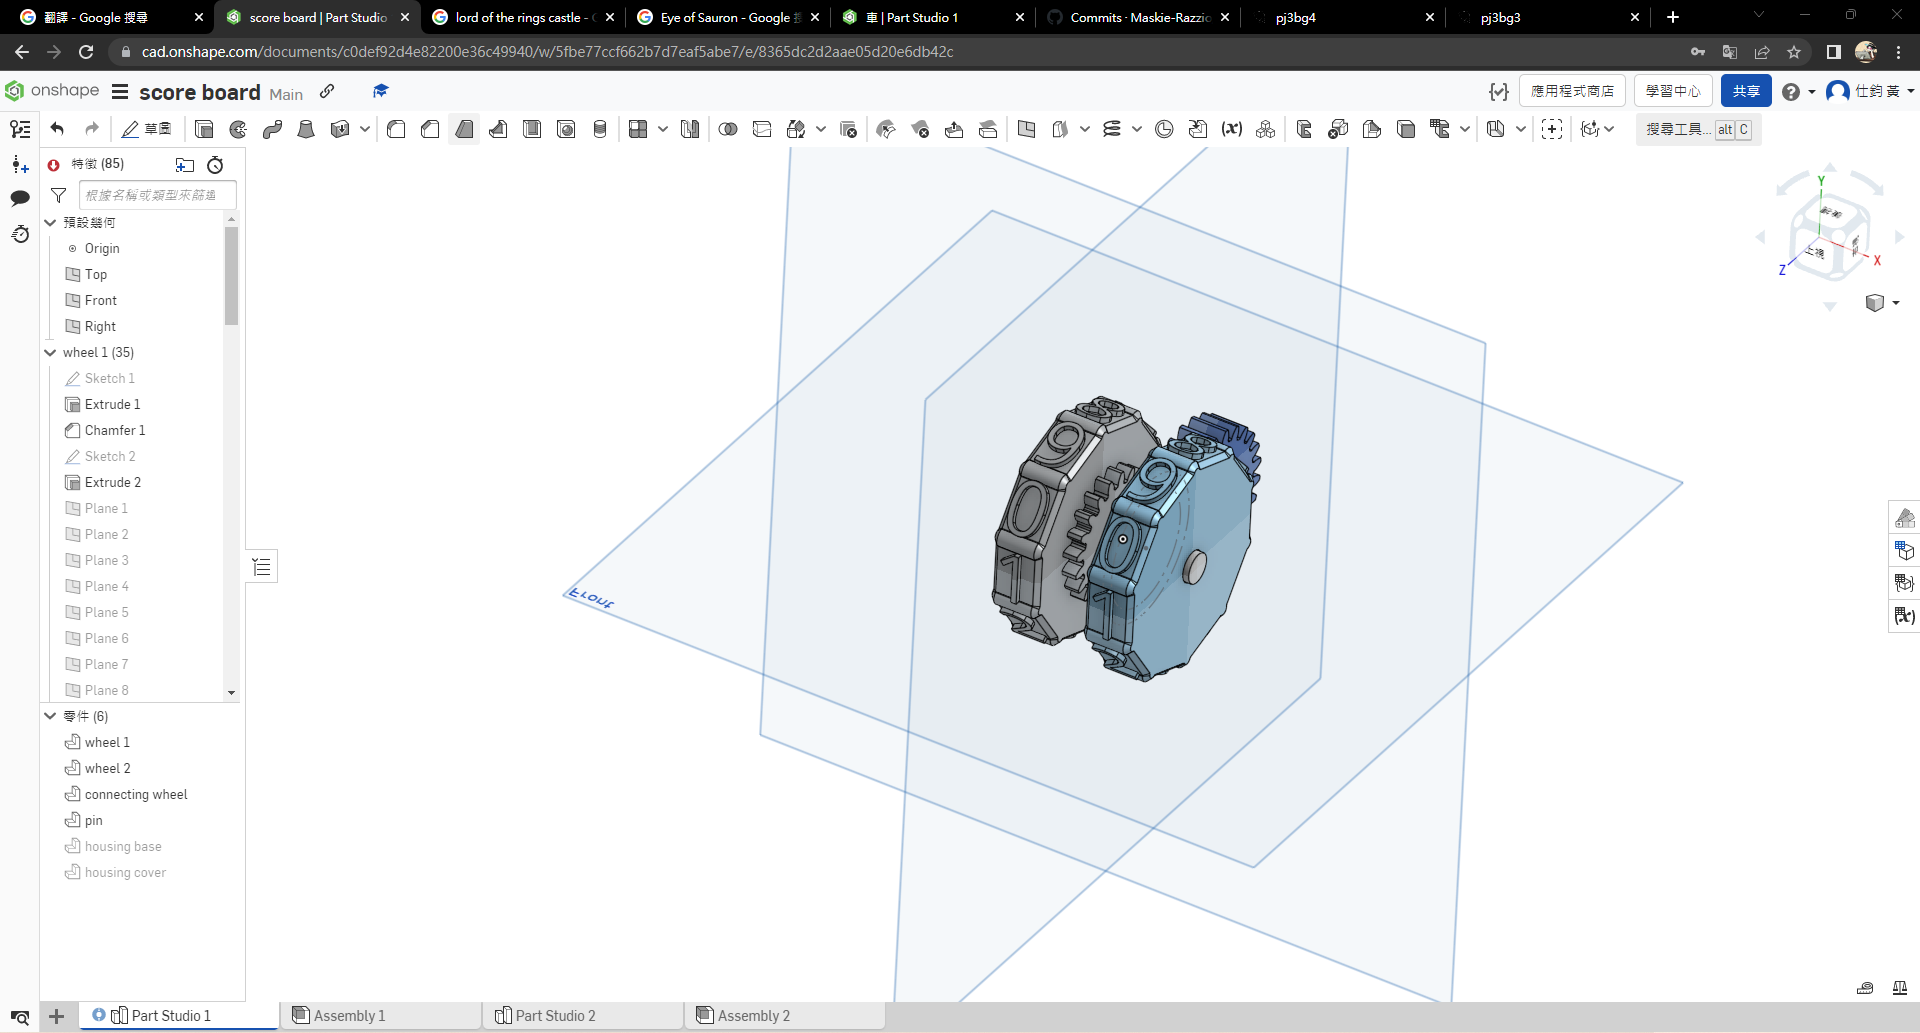
\includegraphics[width=0.5\textwidth]{timer2.png}
  \caption{次代記分板設計圖2}
  \label{fig:example}
\end{figure}


\begin{figure}
  \centering
  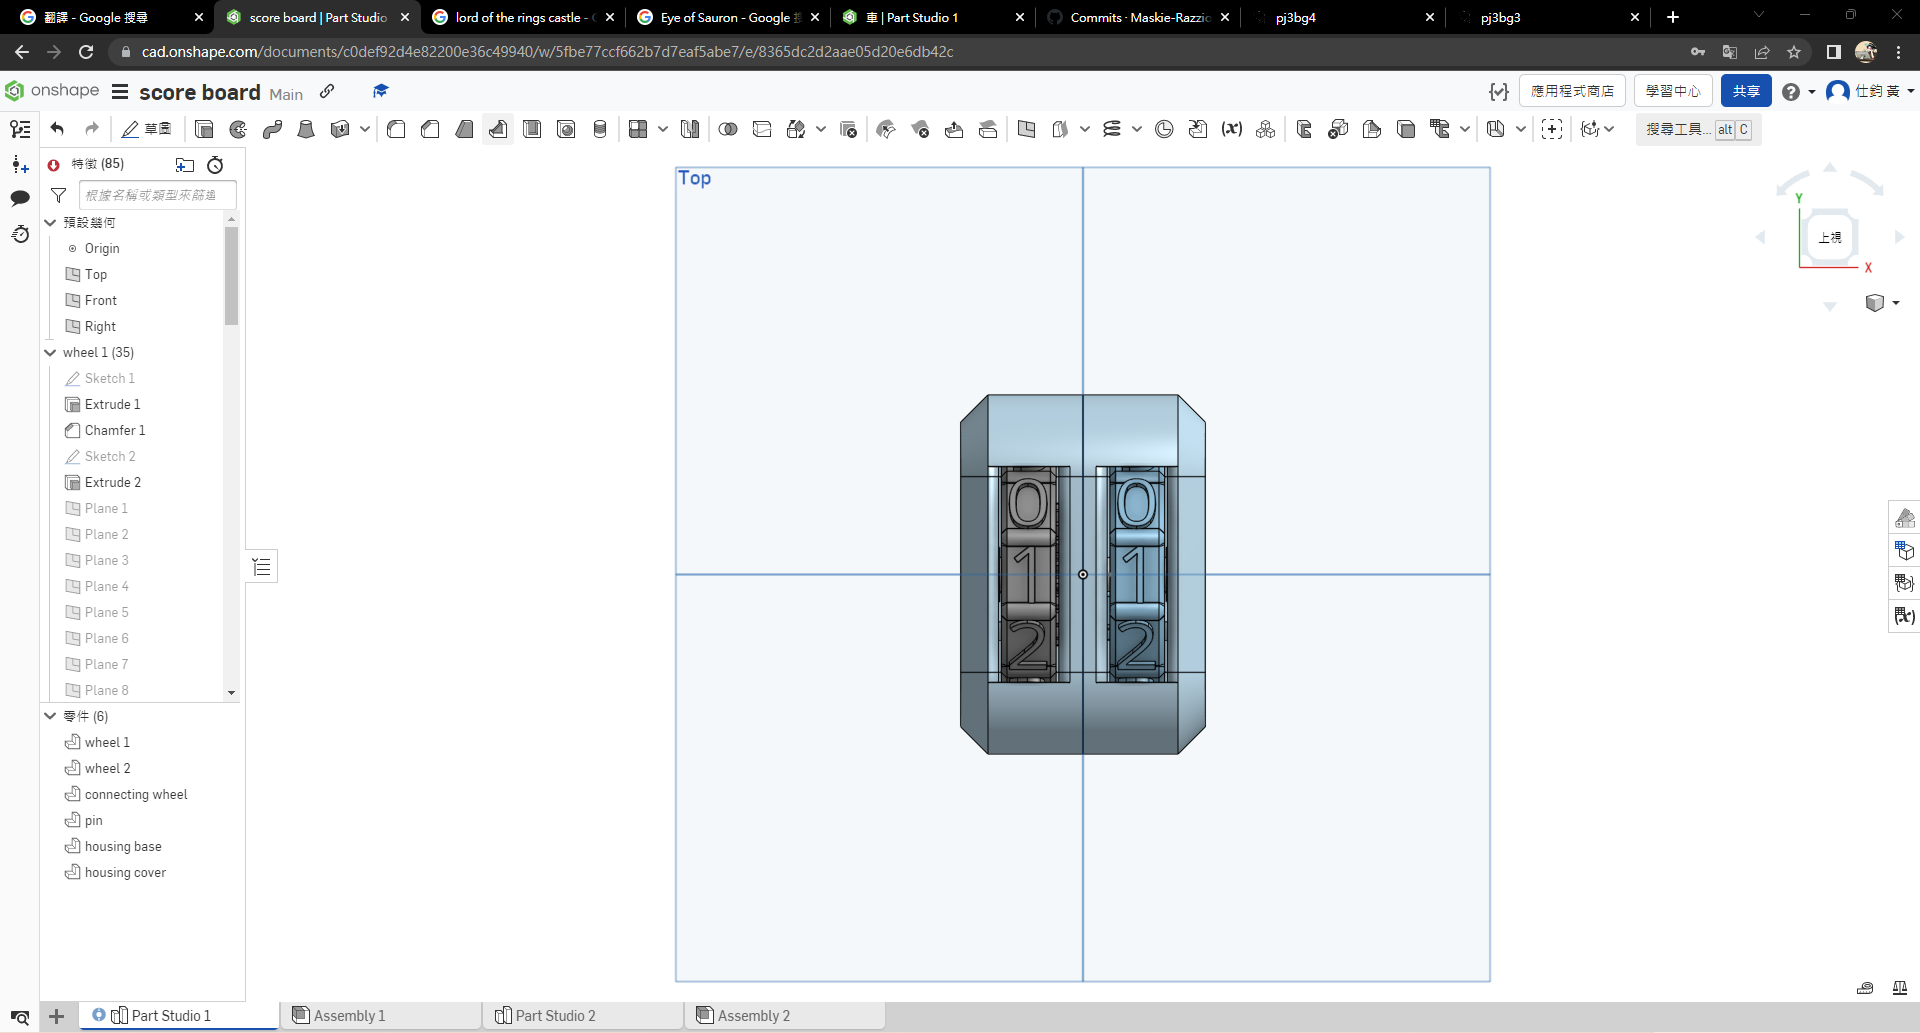
\includegraphics[width=0.5\textwidth]{timer3.png}
  \caption{次代記分板設計圖3}
  \label{fig:example}
\end{figure}


\begin{figure}
  \centering
  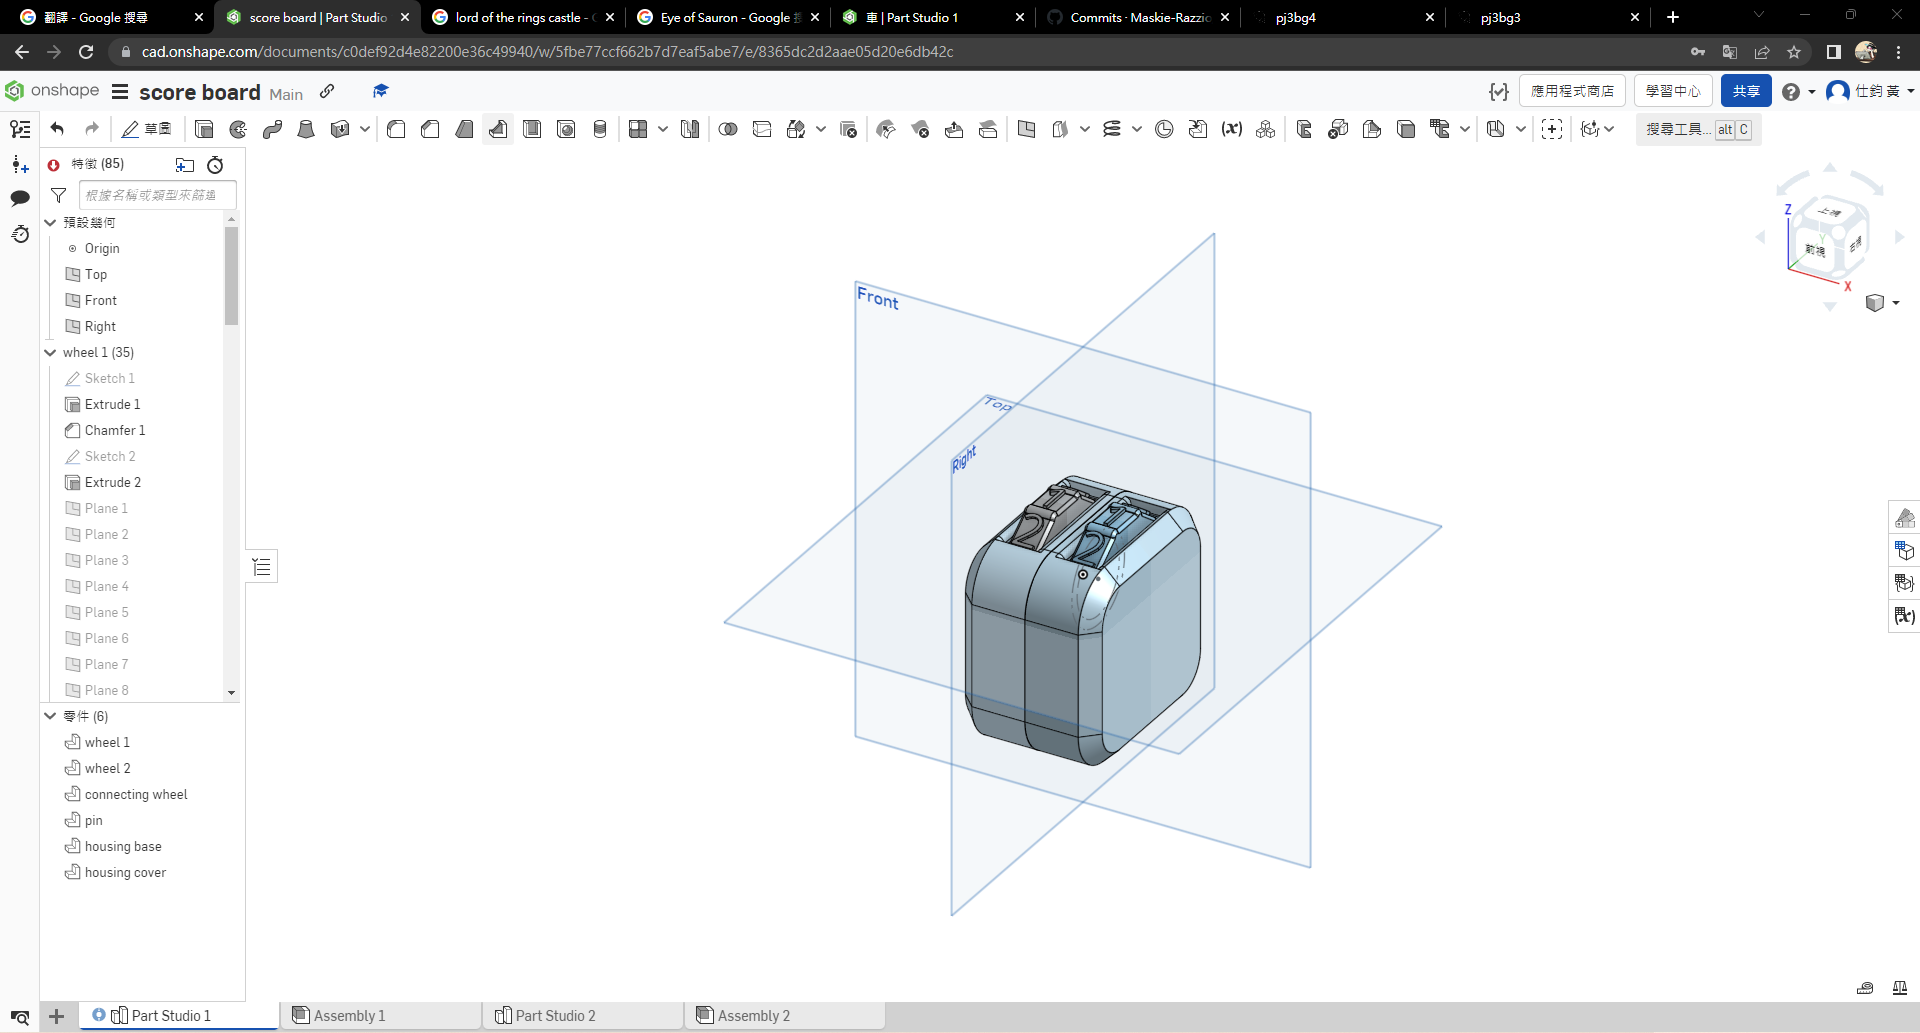
\includegraphics[width=0.5\textwidth]{timer4.png}
  \caption{次代記分板設計圖4}
  \label{fig:example}
\end{figure}


\begin{figure}
  \centering
  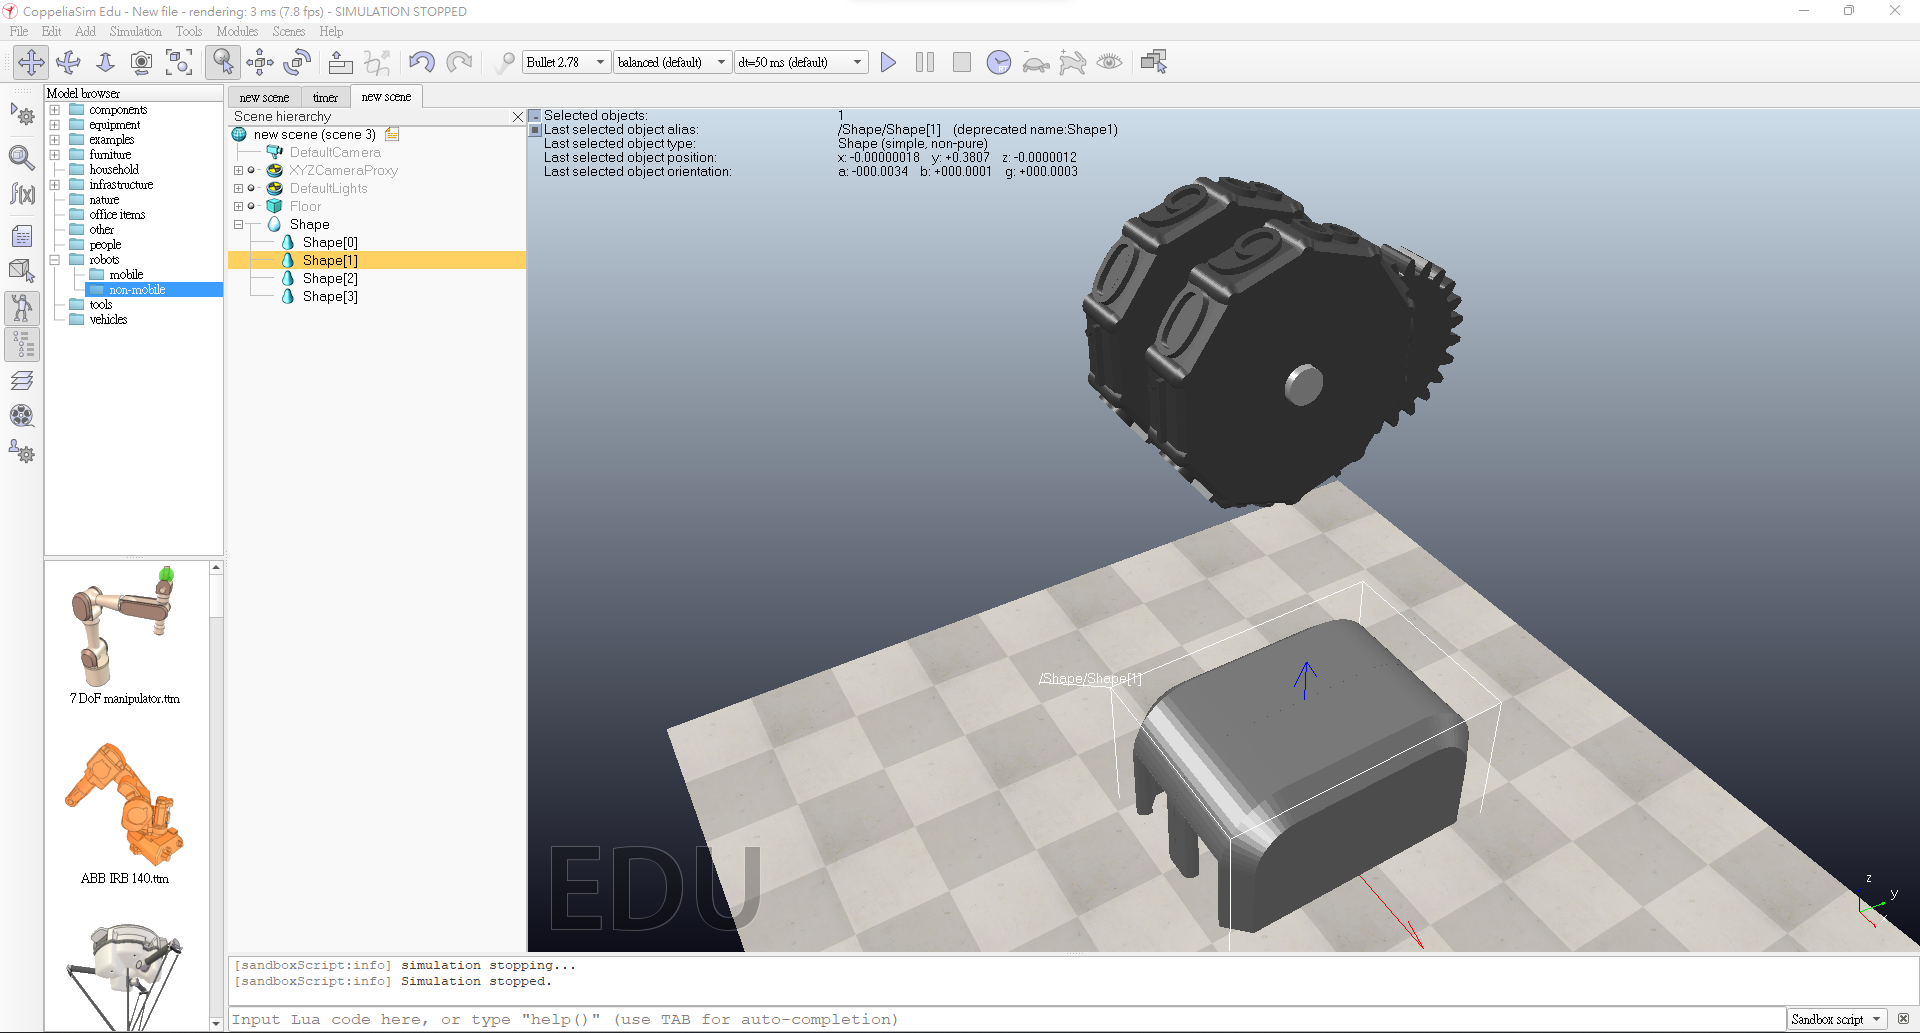
\includegraphics[width=0.5\textwidth]{timer1.0-1.png}
  \caption{次代記分板設計圖5}
  \label{fig:example}
\end{figure}


\begin{figure}
  \centering
  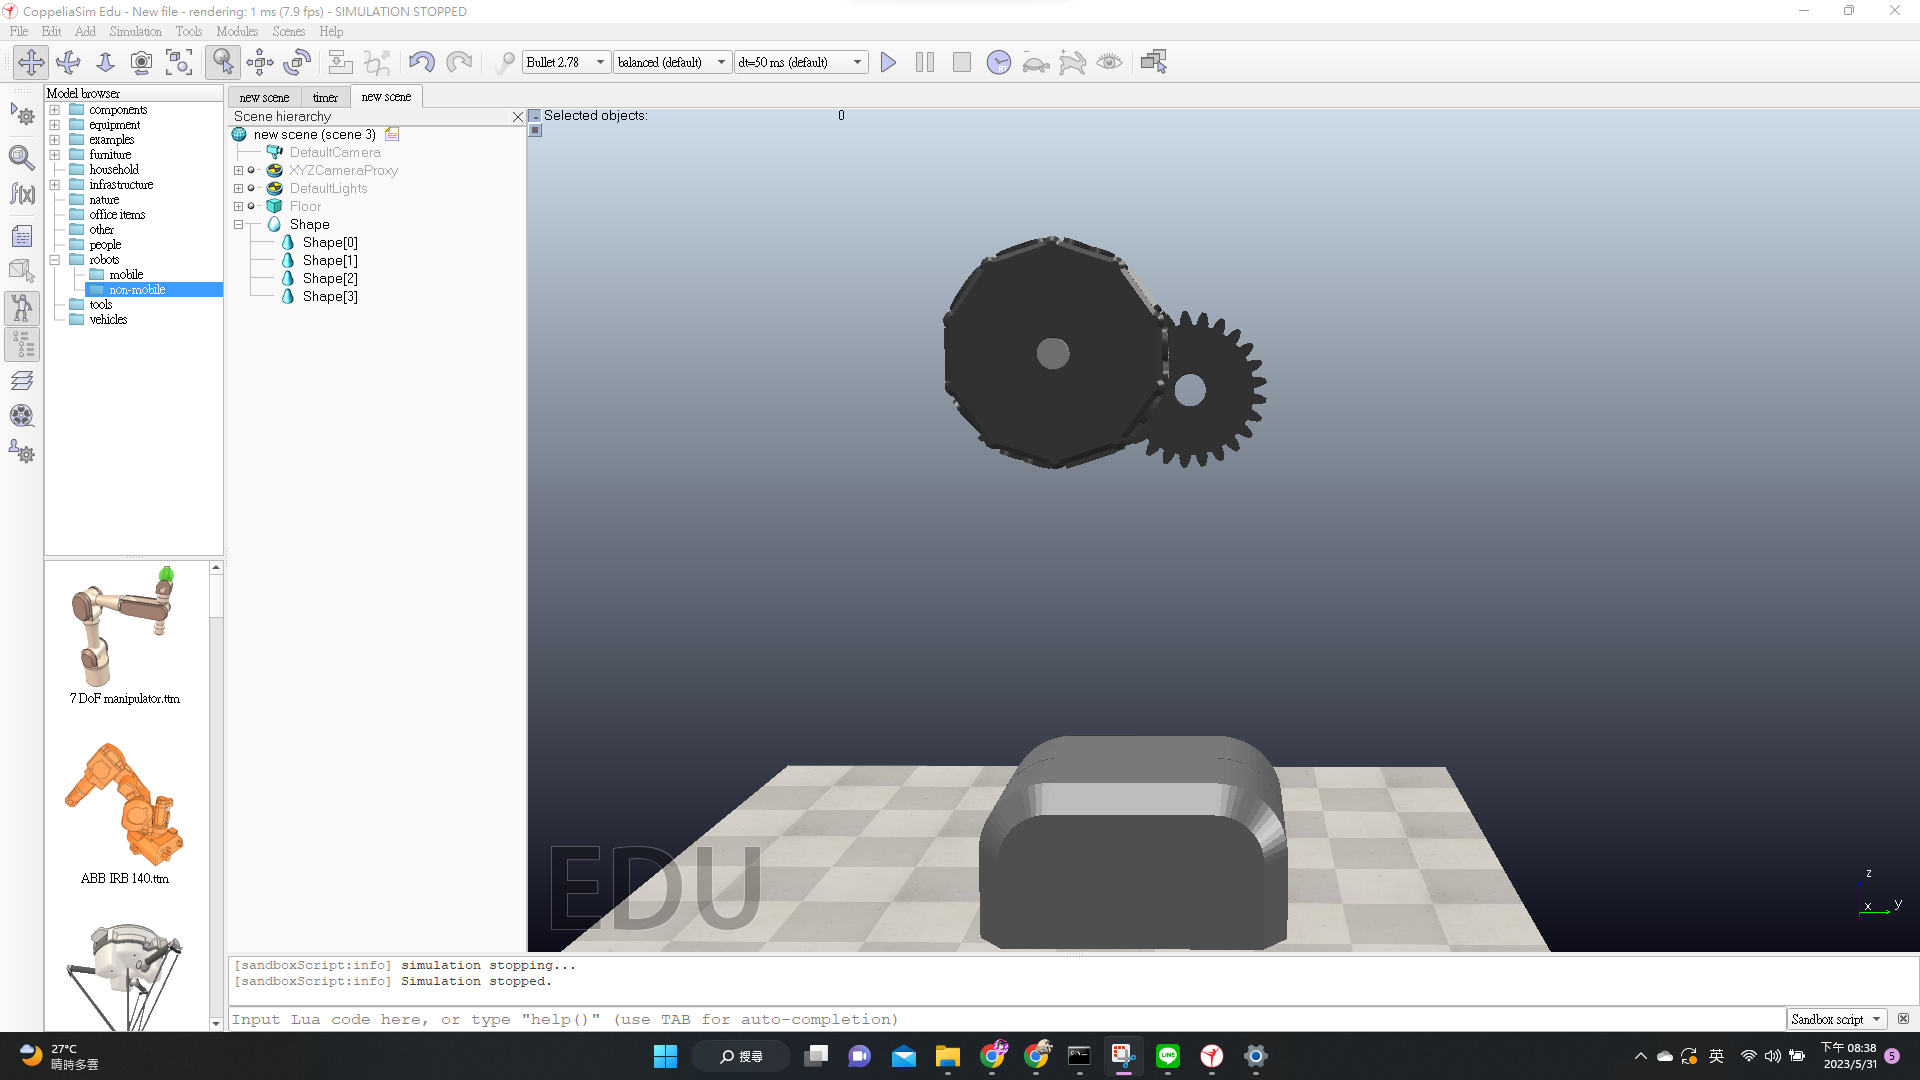
\includegraphics[width=0.5\textwidth]{timer1.0-3.png}
  \caption{次代記分板設計圖6}
  \label{fig:example}
\end{figure}


\begin{figure}
  \centering
  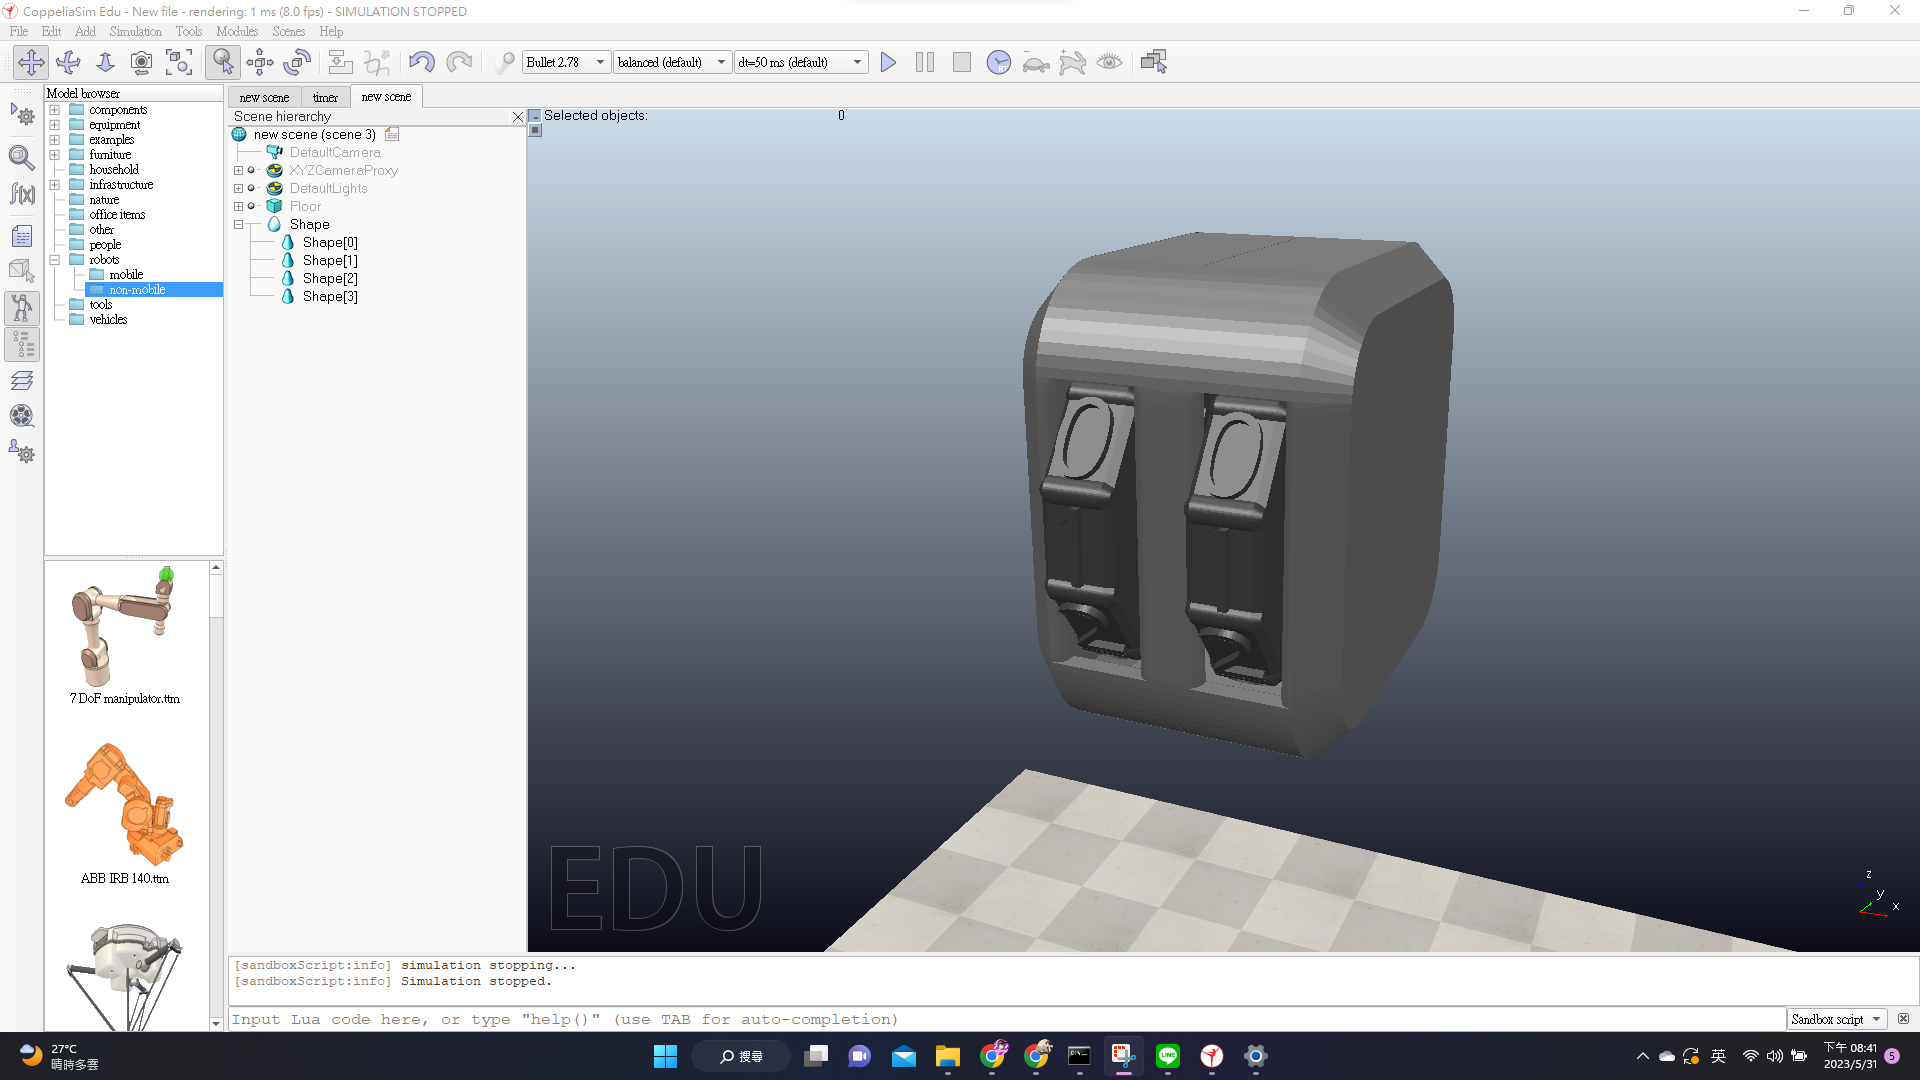
\includegraphics[width=0.5\textwidth]{timer1.0-5.png}
  \caption{次代記分板設計圖7}
  \label{fig:example}
\end{figure}


\begin{figure}
  \centering
  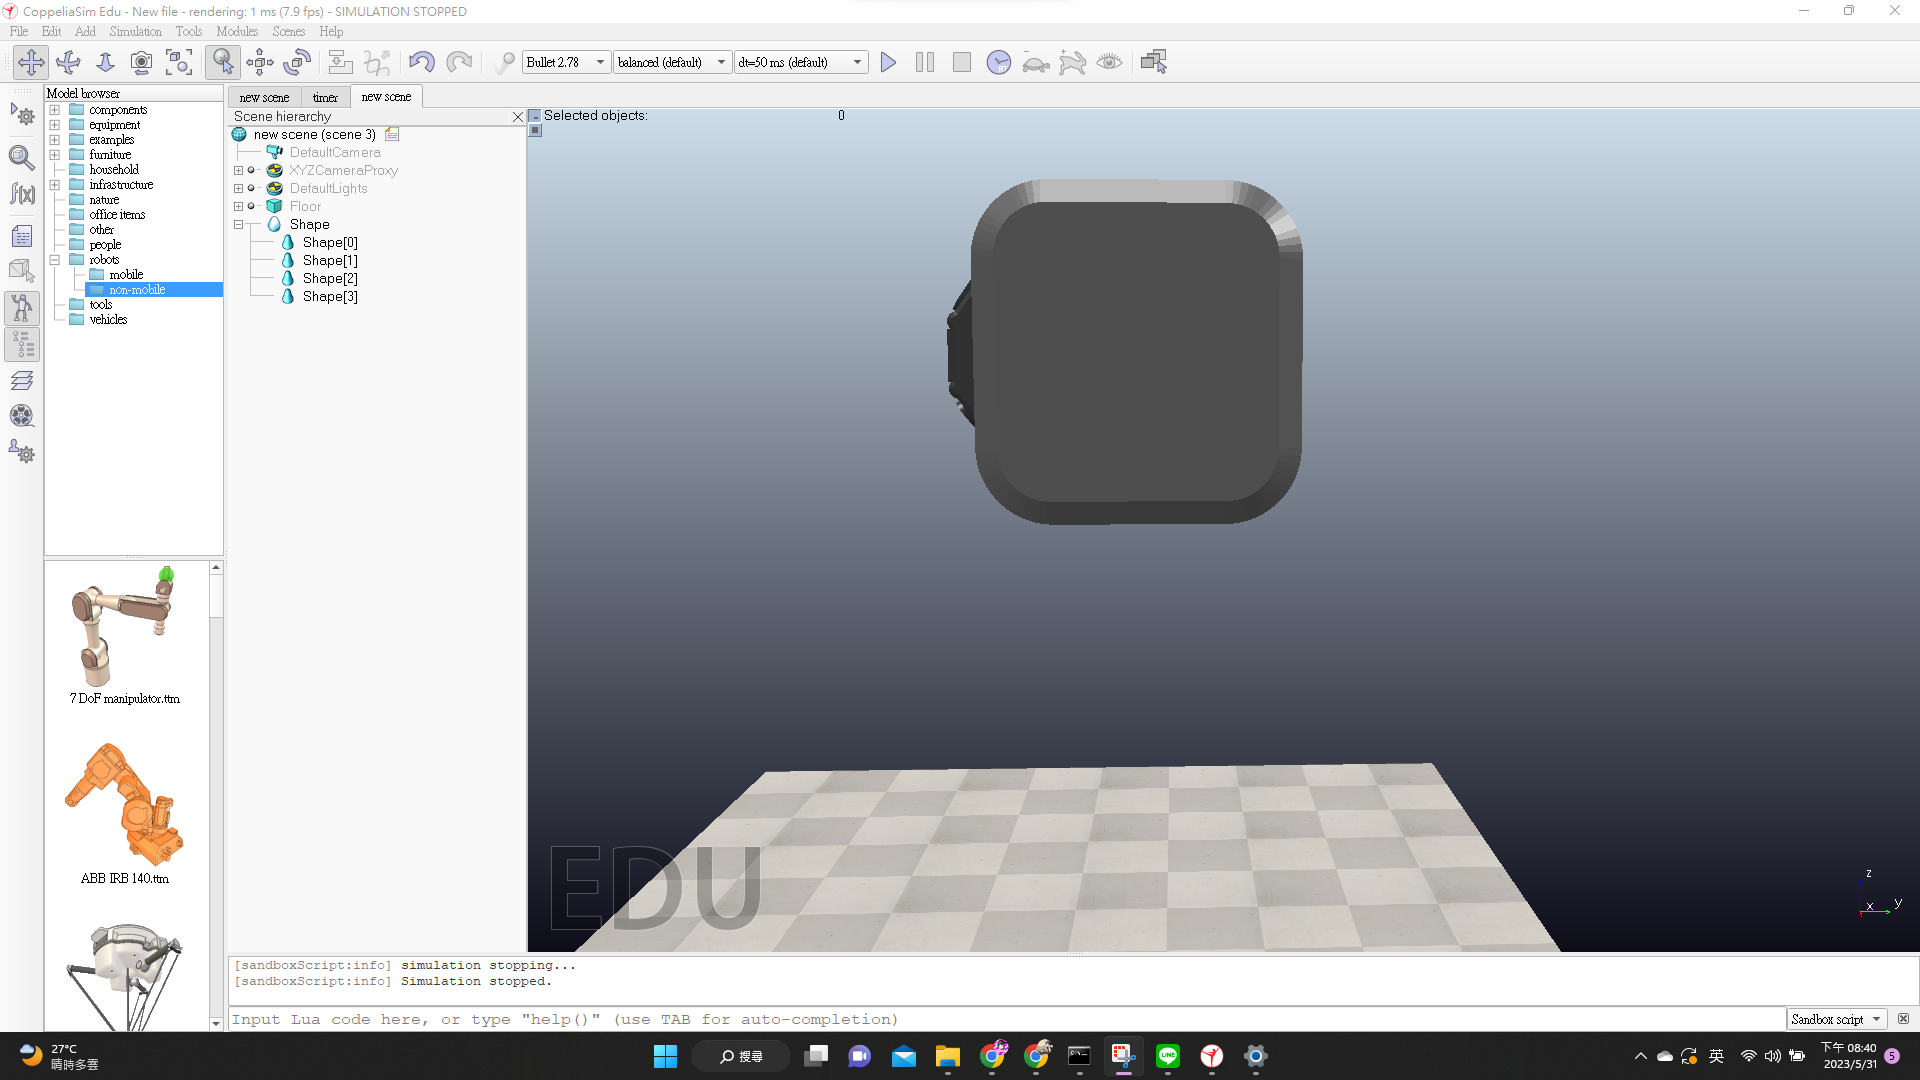
\includegraphics[width=0.5\textwidth]{timer1.0-4.png}
  \caption{次代記分板設計圖8}
  \label{fig:example}
\end{figure}


\begin{figure}
  \centering
  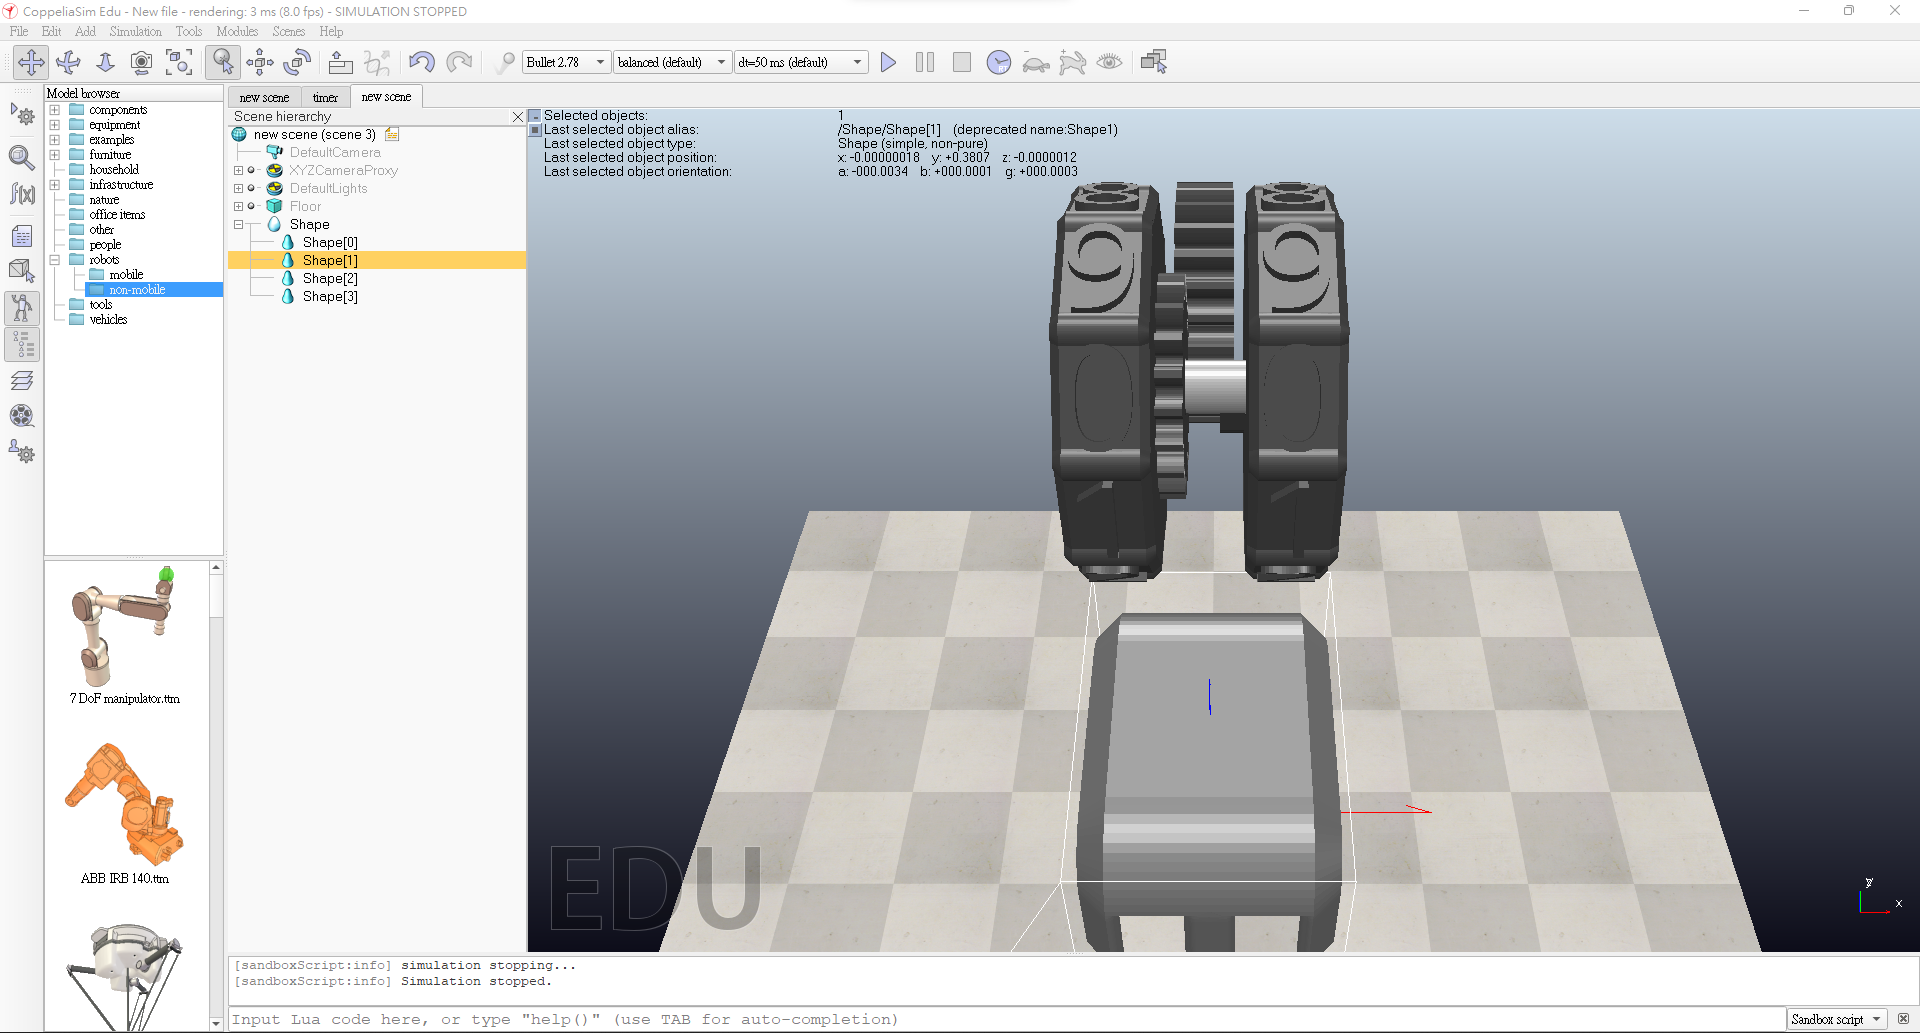
\includegraphics[width=0.5\textwidth]{timer1.0-2.png}
  \caption{次代記分板設計圖9}
  \label{fig:example}
\end{figure}



三代的數字都改模成新版的個別分件,通過平面配合各自組裝,使其可更加明顯,且外殼多擴兩孔、齒輪微調和增加輔助軸,使輪盤更方便抓到支點且連動更順滑,雖然變化看起來不大但總體表現都有一定更新


\begin{figure}
  \centering
  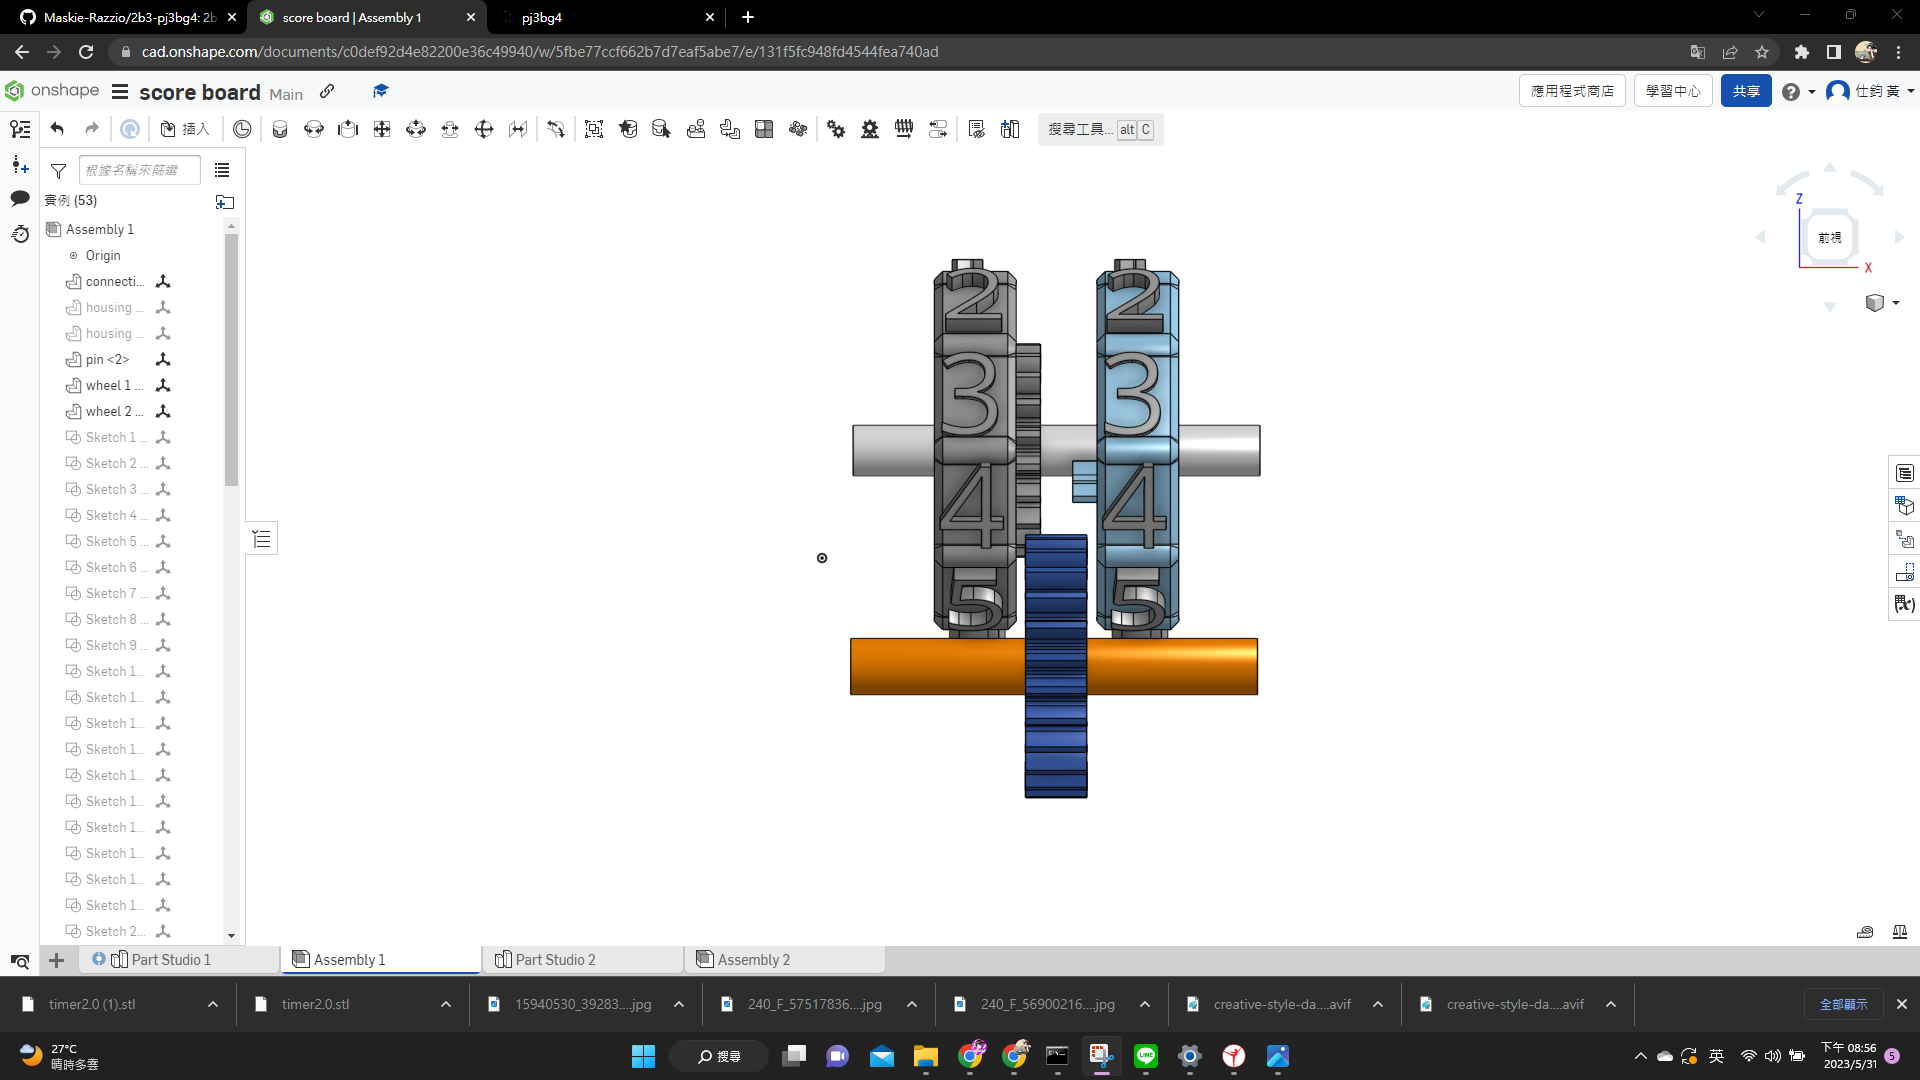
\includegraphics[width=0.5\textwidth]{timer10.png}
  \caption{三代記分板設計圖1}
  \label{fig:example}
\end{figure}


\begin{figure}
  \centering
  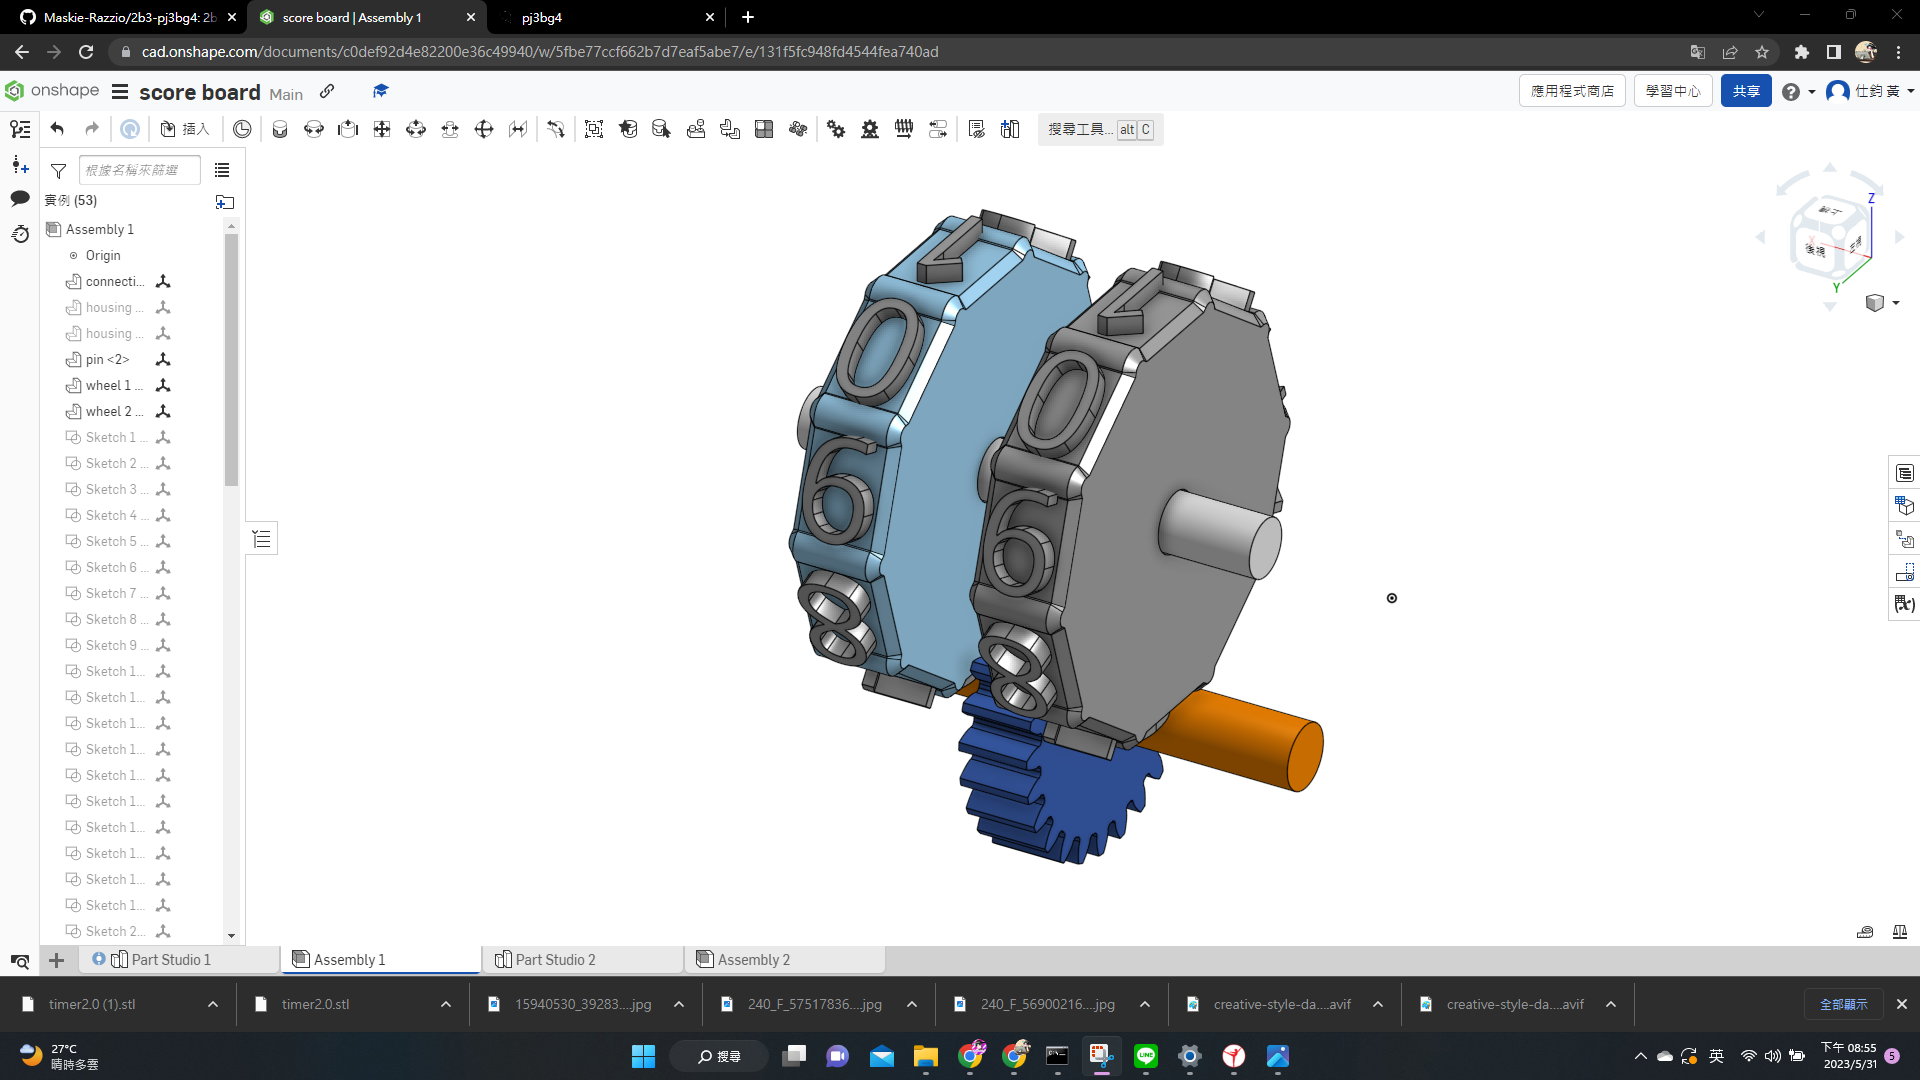
\includegraphics[width=0.5\textwidth]{timer9.png}
  \caption{三代記分板設計圖2}
  \label{fig:example}
\end{figure}


\begin{figure}
  \centering
  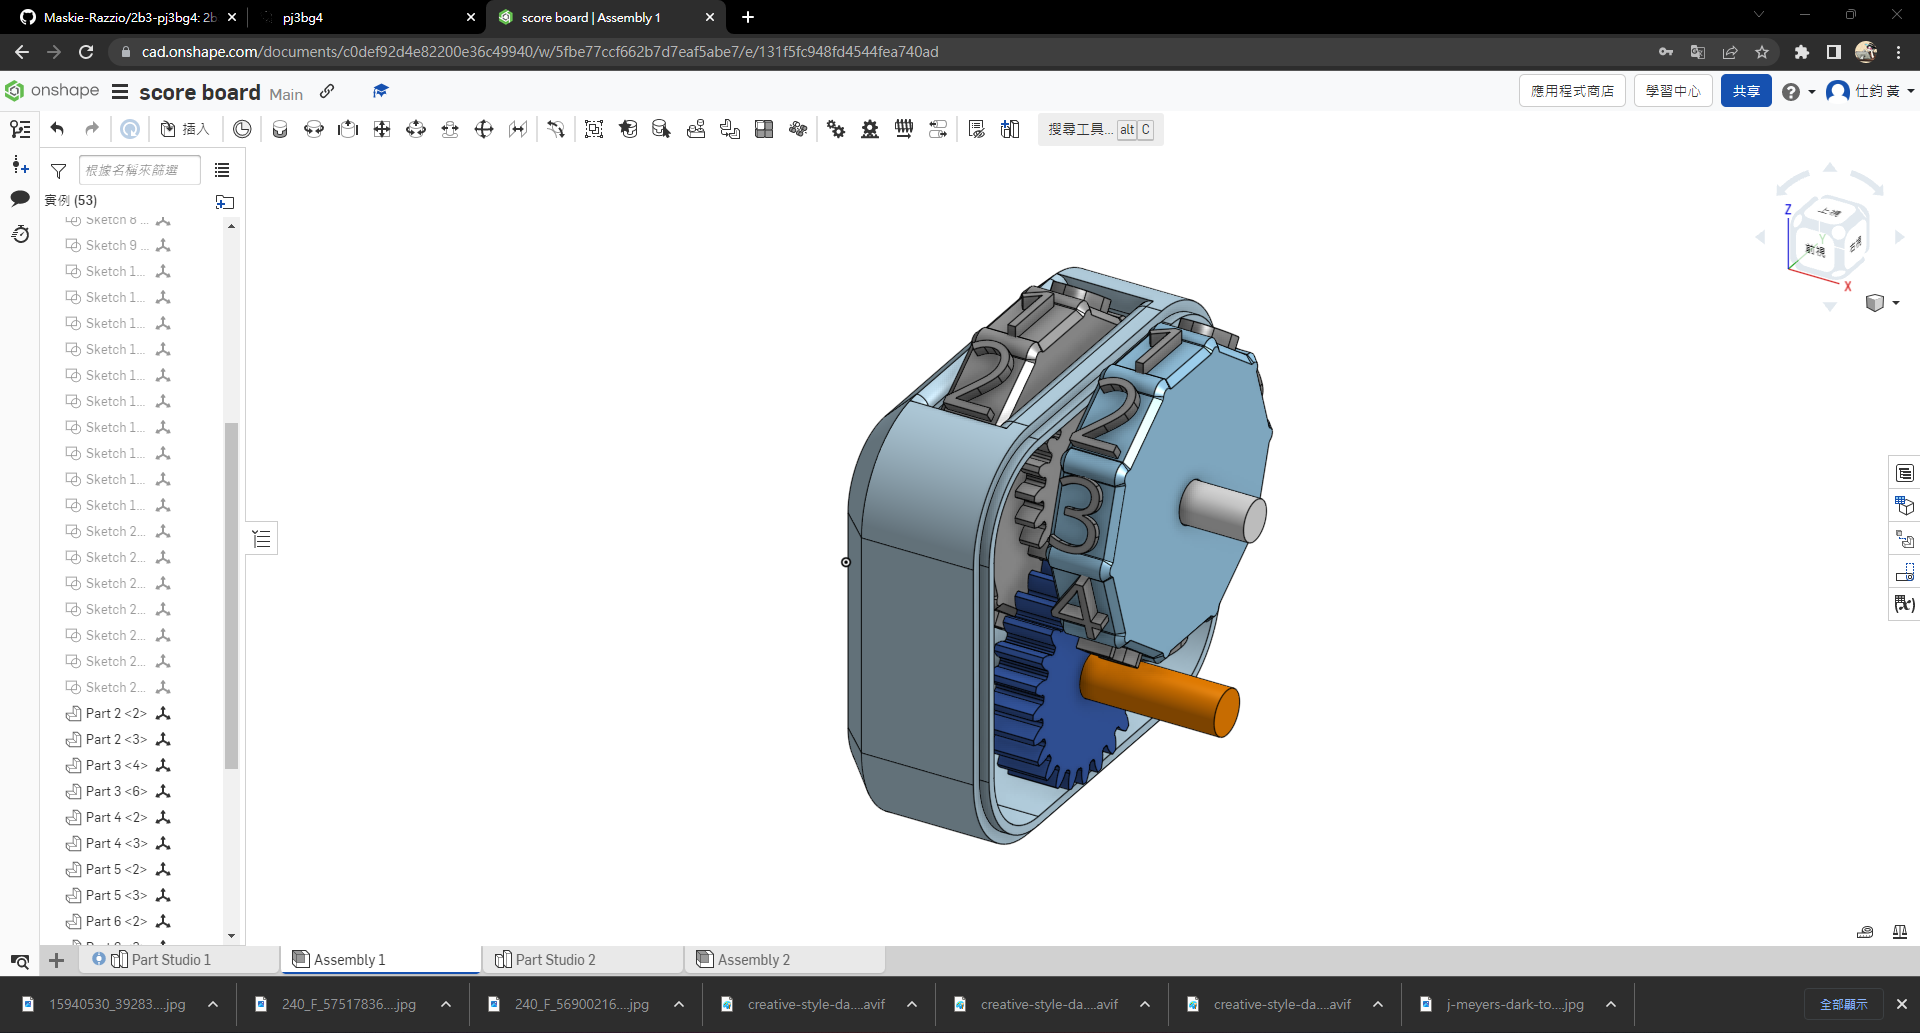
\includegraphics[width=0.5\textwidth]{timer5.png}
  \caption{三代記分板設計圖3}
  \label{fig:example}
\end{figure}


\begin{figure}
  \centering
  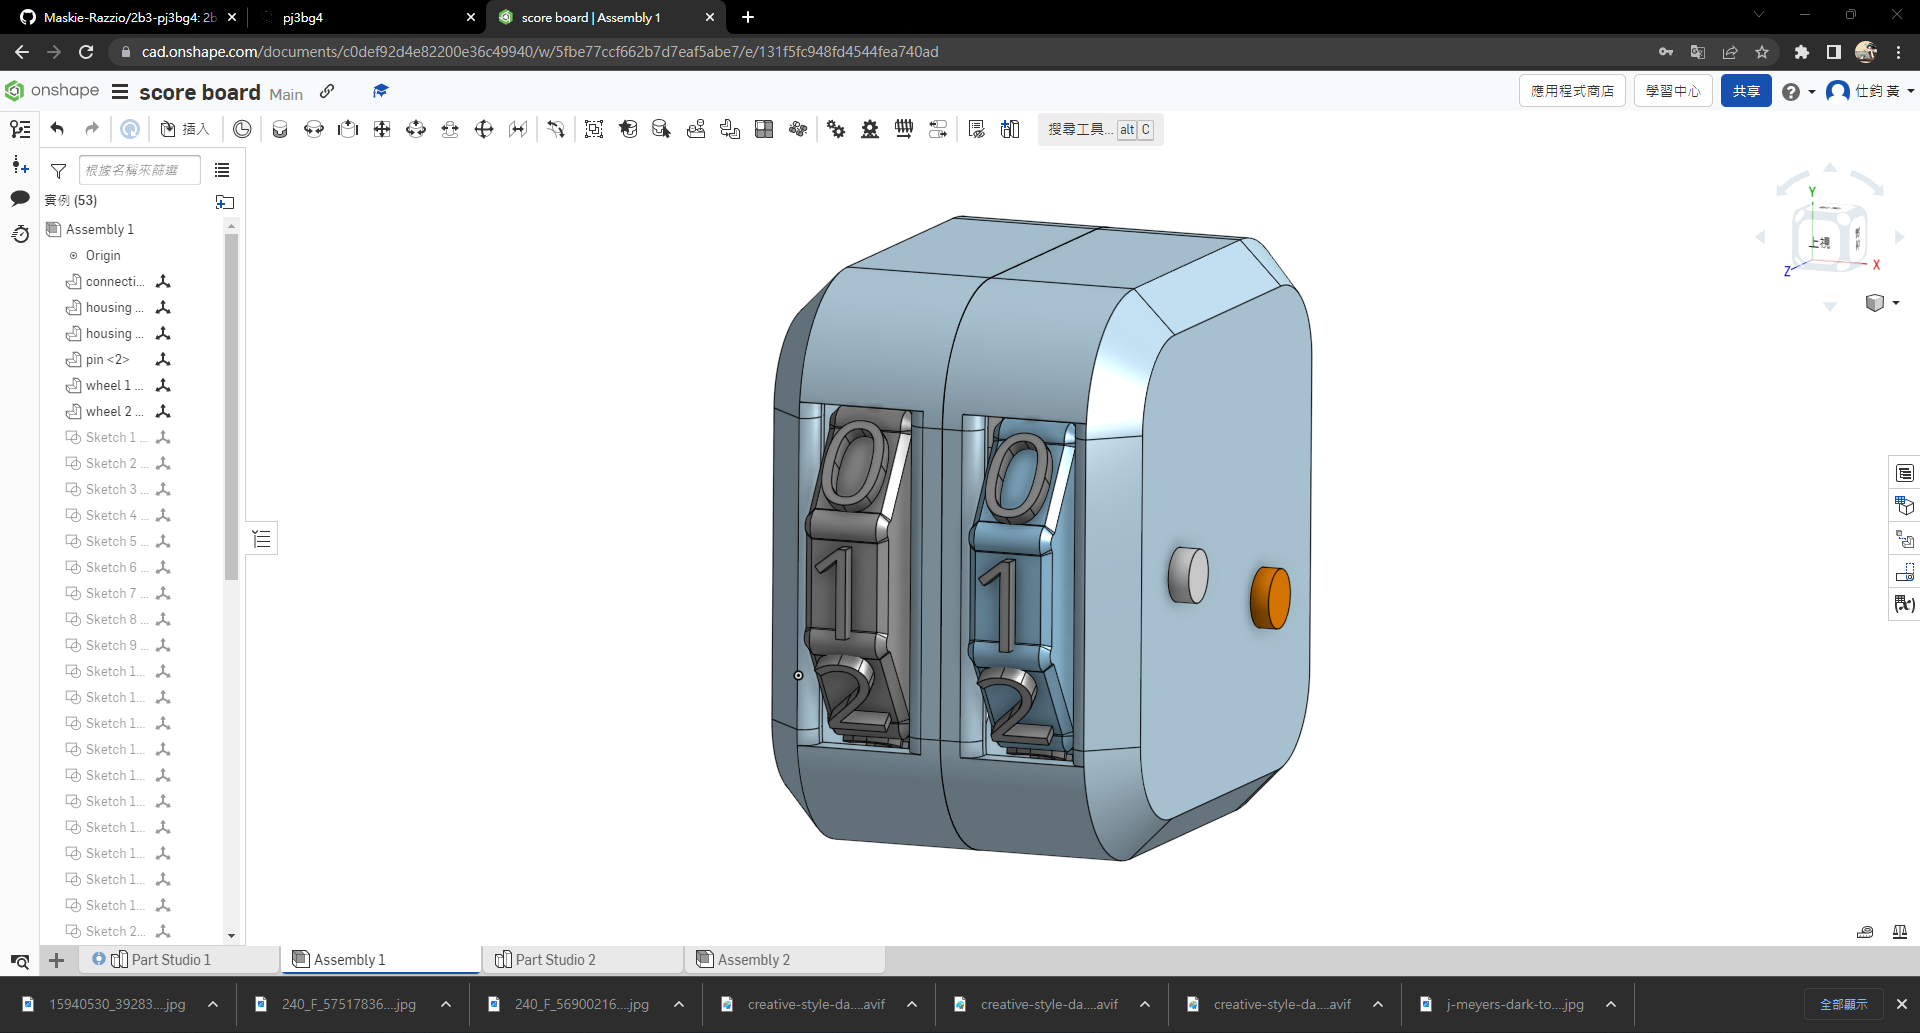
\includegraphics[width=0.5\textwidth]{timer6.png}
  \caption{三代記分板設計圖4}
  \label{fig:example}
\end{figure}


\begin{figure}
  \centering
  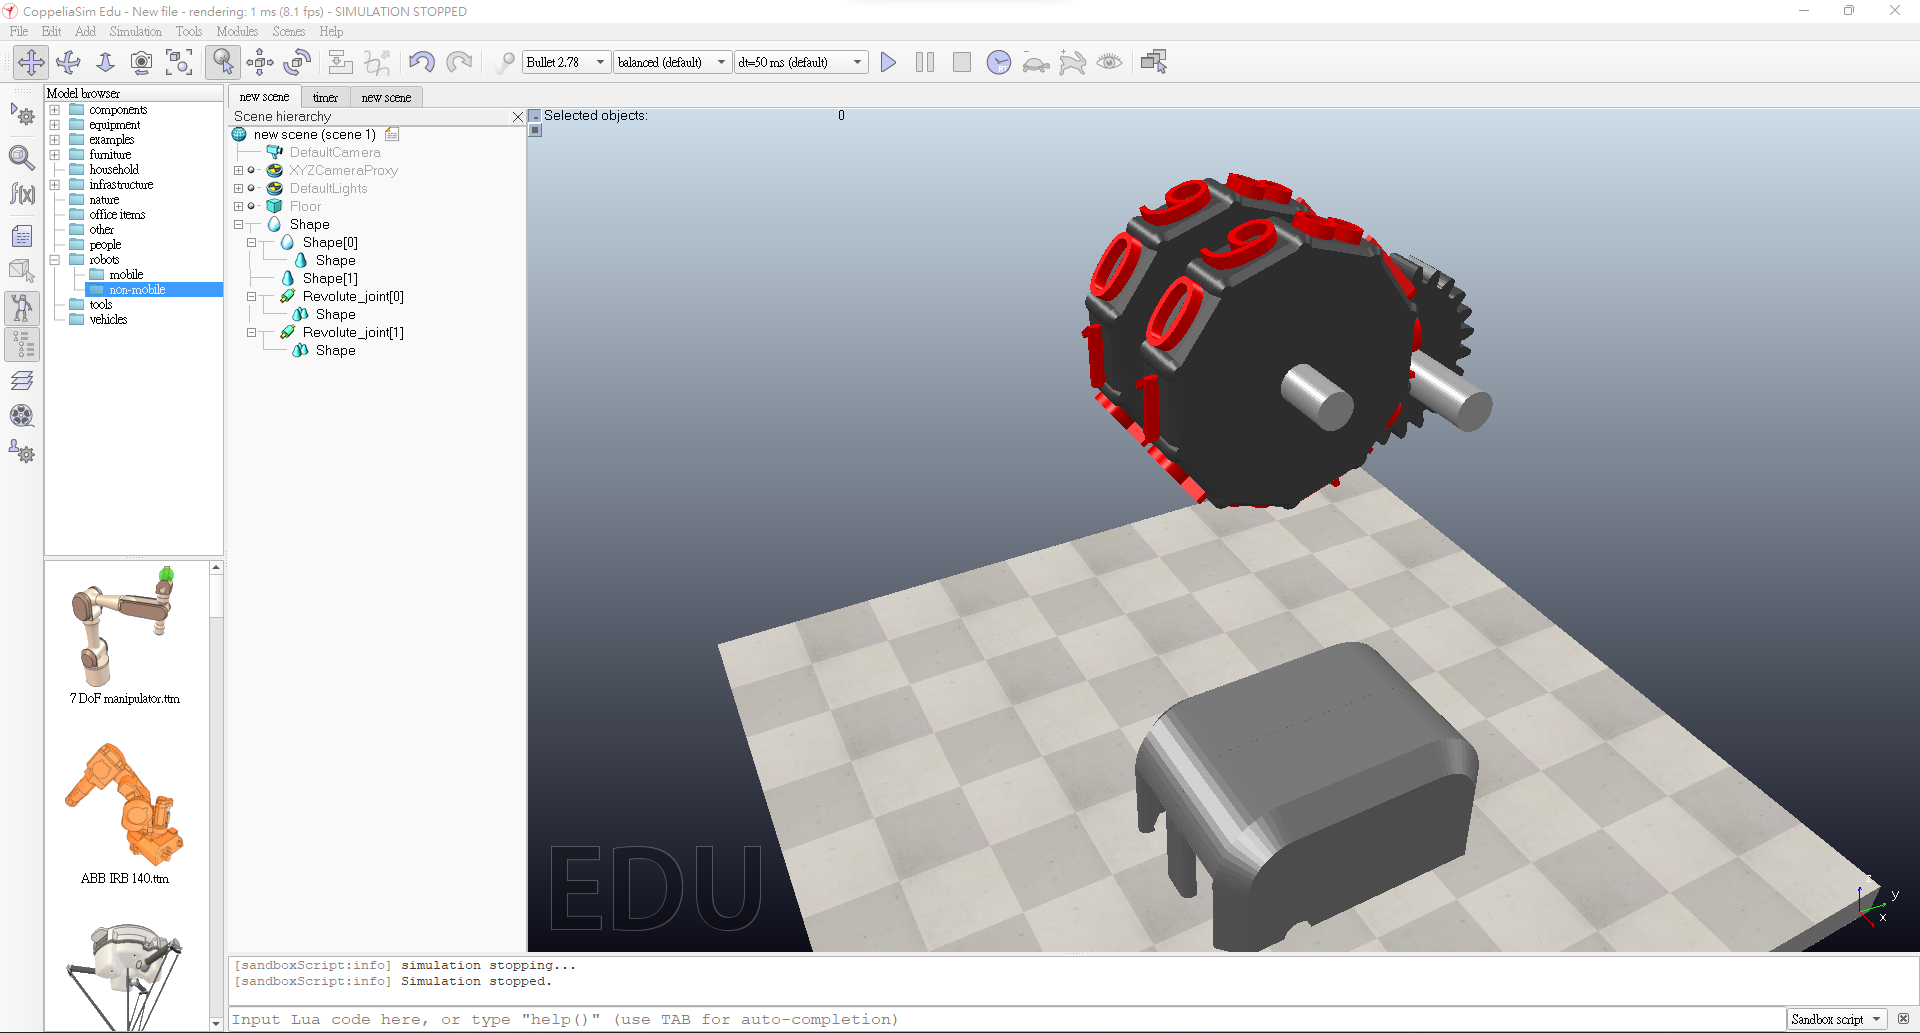
\includegraphics[width=0.5\textwidth]{timer2.0-1.png}
  \caption{三代記分板設計圖5}
  \label{fig:example}
\end{figure}


\begin{figure}
  \centering
  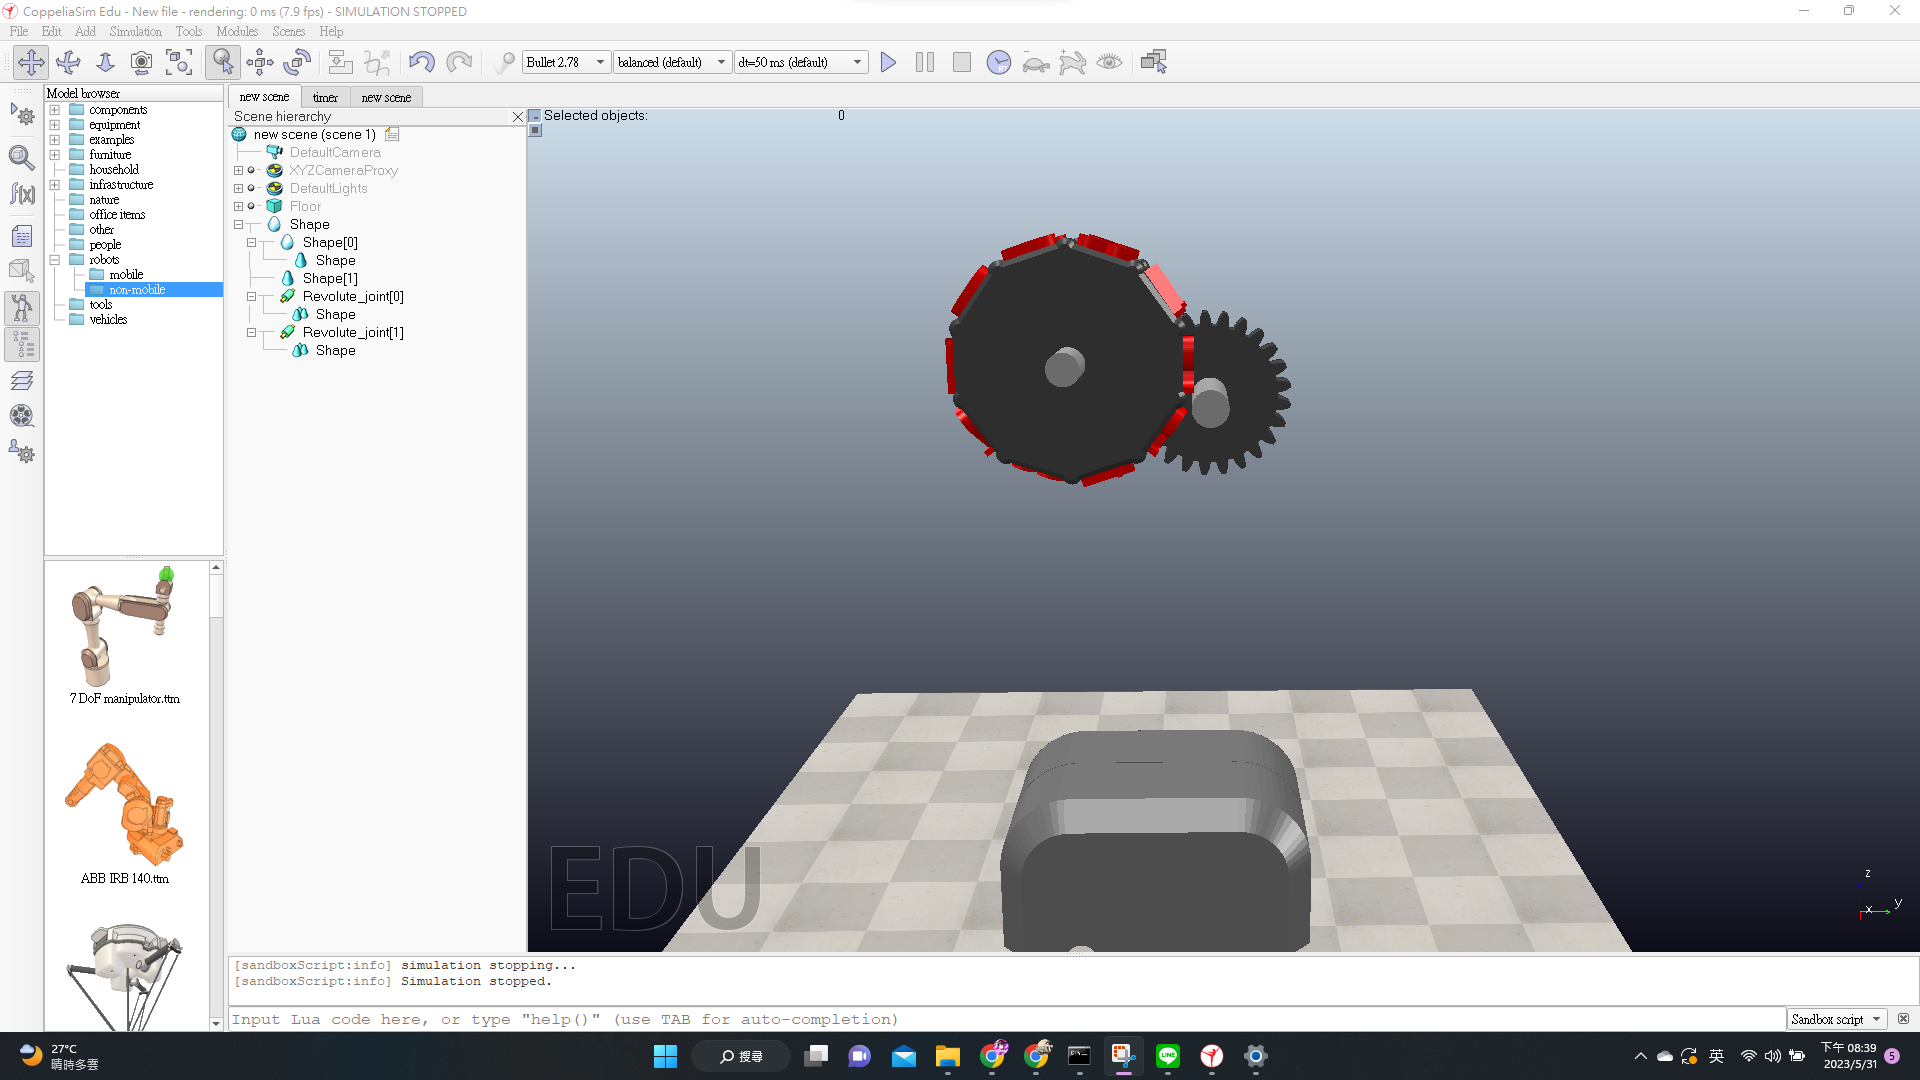
\includegraphics[width=0.5\textwidth]{timer2.0-3.png}
  \caption{三代記分板設計圖6}
  \label{fig:example}
\end{figure}


\begin{figure}
  \centering
  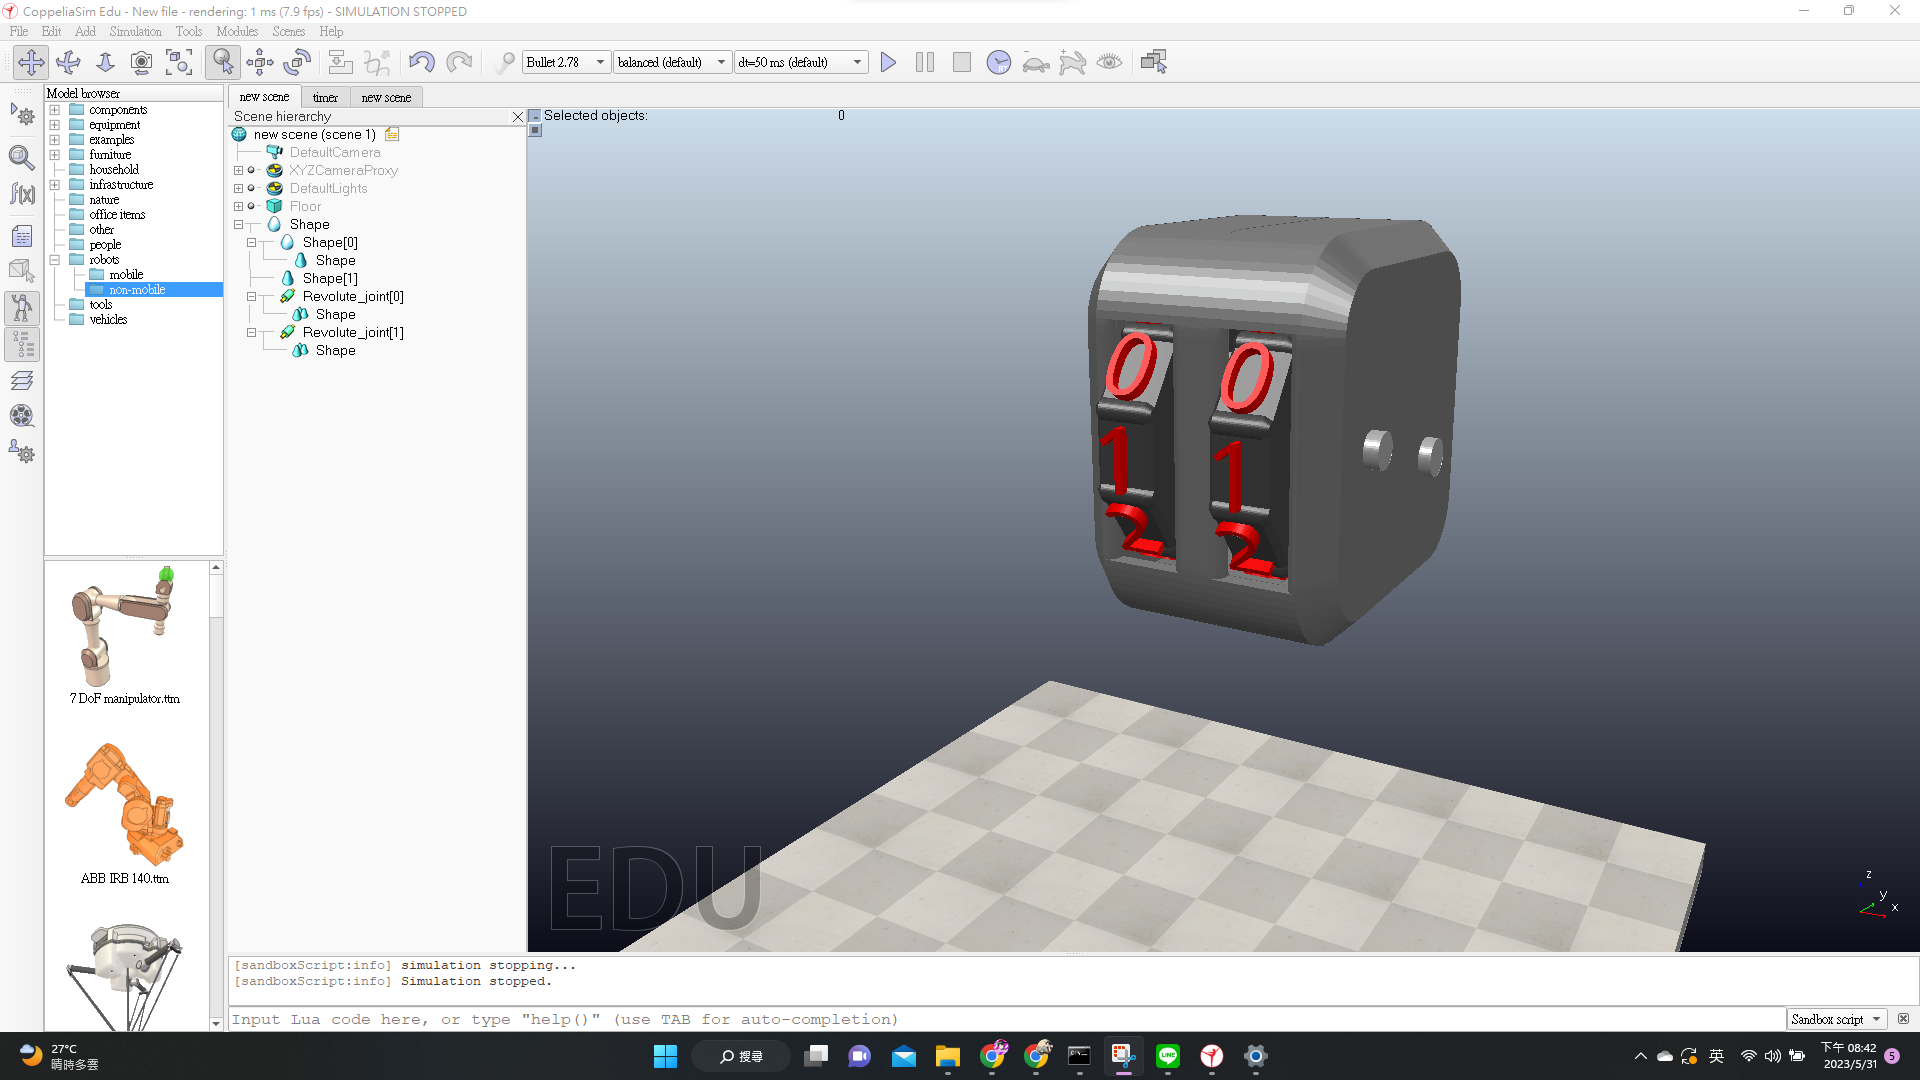
\includegraphics[width=0.5\textwidth]{timer2.0-5.png}
  \caption{三代記分板設計圖7}
  \label{fig:example}
\end{figure}


\begin{figure}
  \centering
  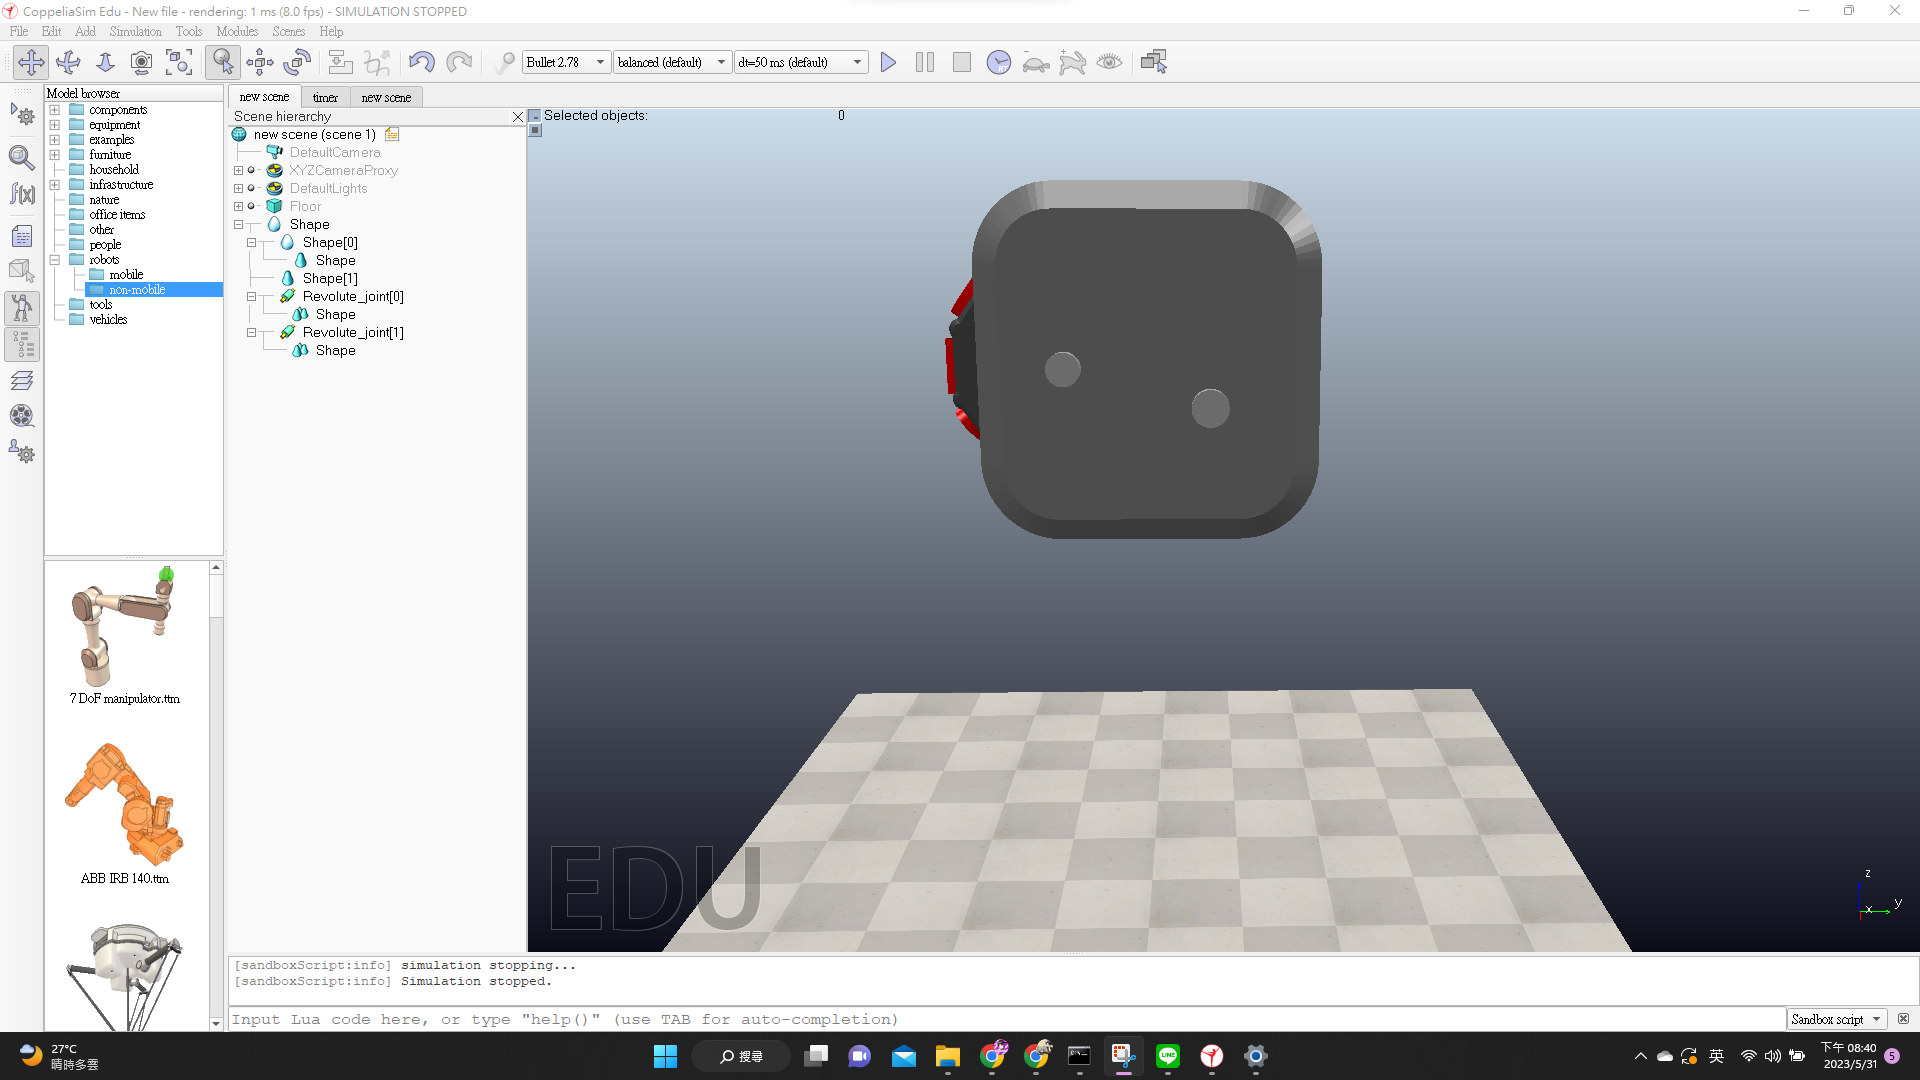
\includegraphics[width=0.5\textwidth]{timer2.0-4.png}
  \caption{三代記分板設計圖8}
  \label{fig:example}
\end{figure}


\begin{figure}
  \centering
  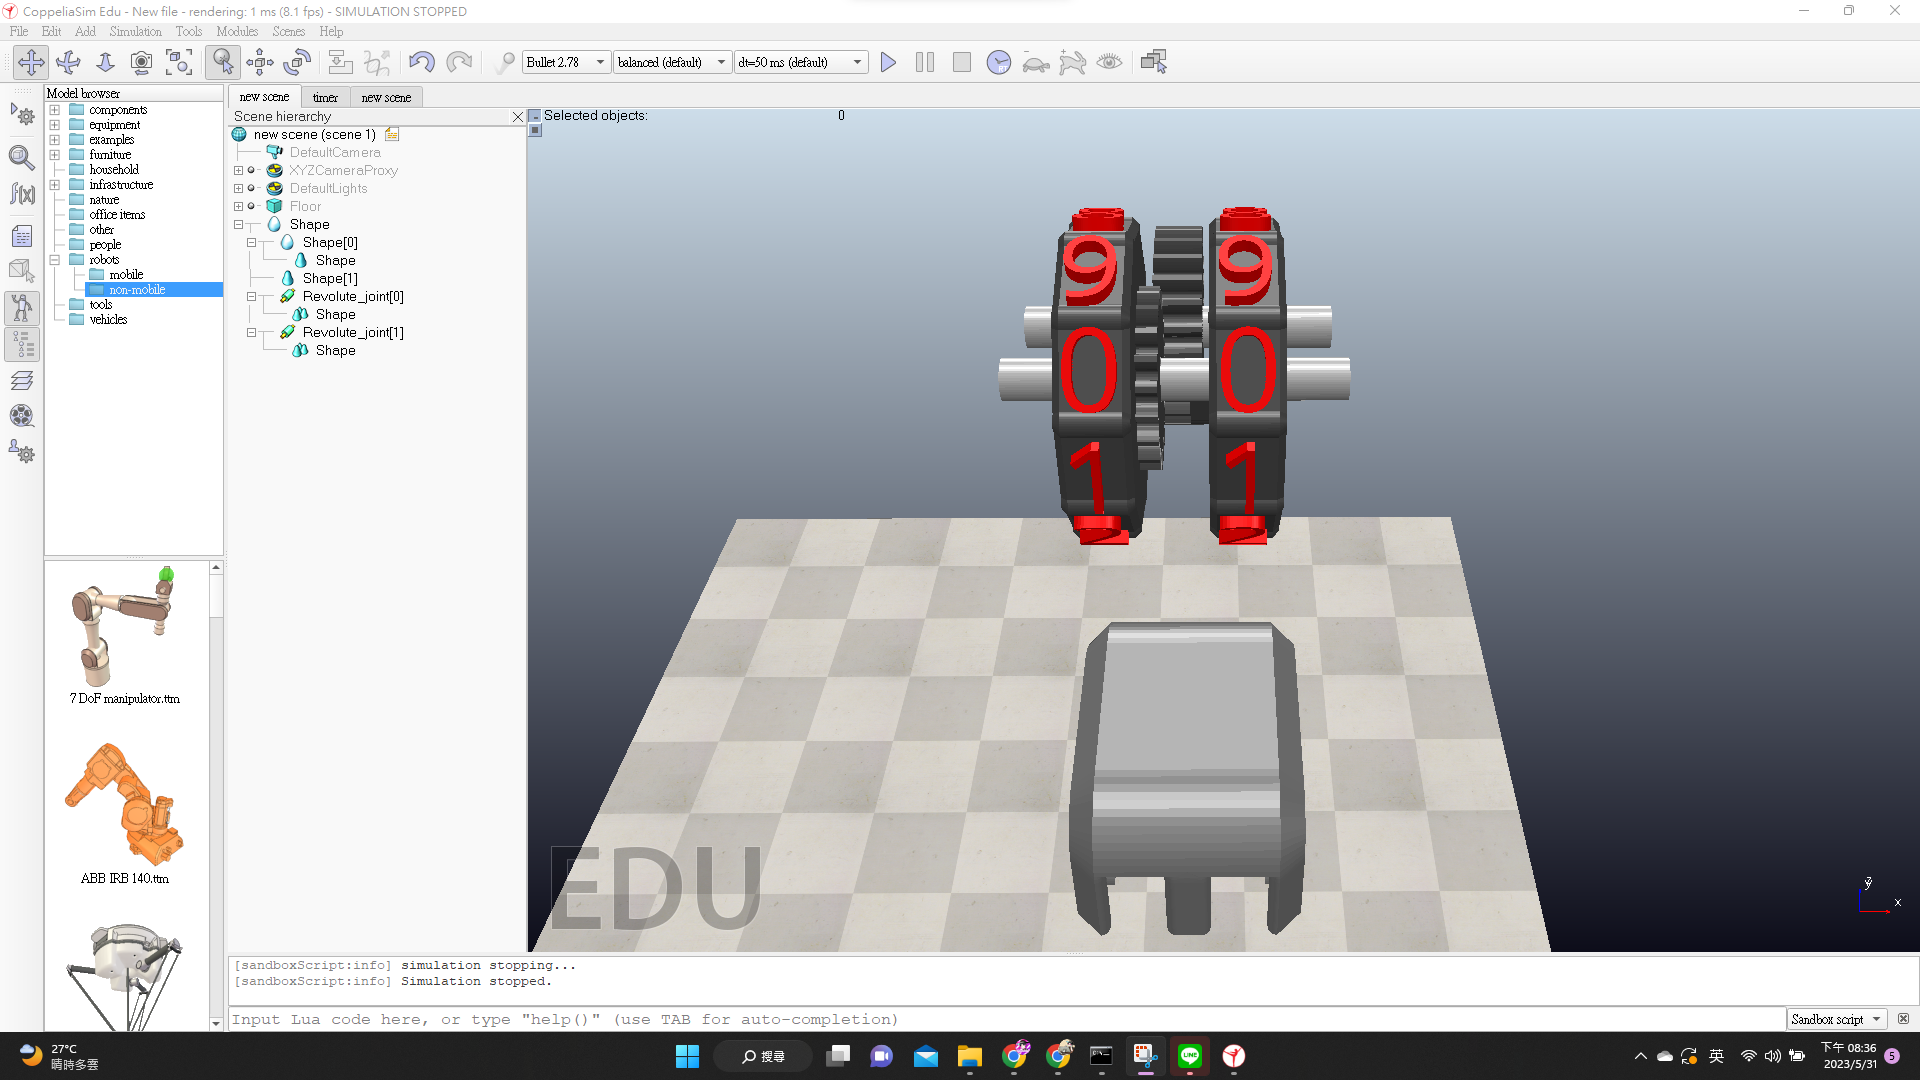
\includegraphics[width=0.5\textwidth]{timer2.0-2.png}
  \caption{三代記分板設計圖9}
  \label{fig:example}
\end{figure}

\section{球場}

\begin{figure}
  \centering
  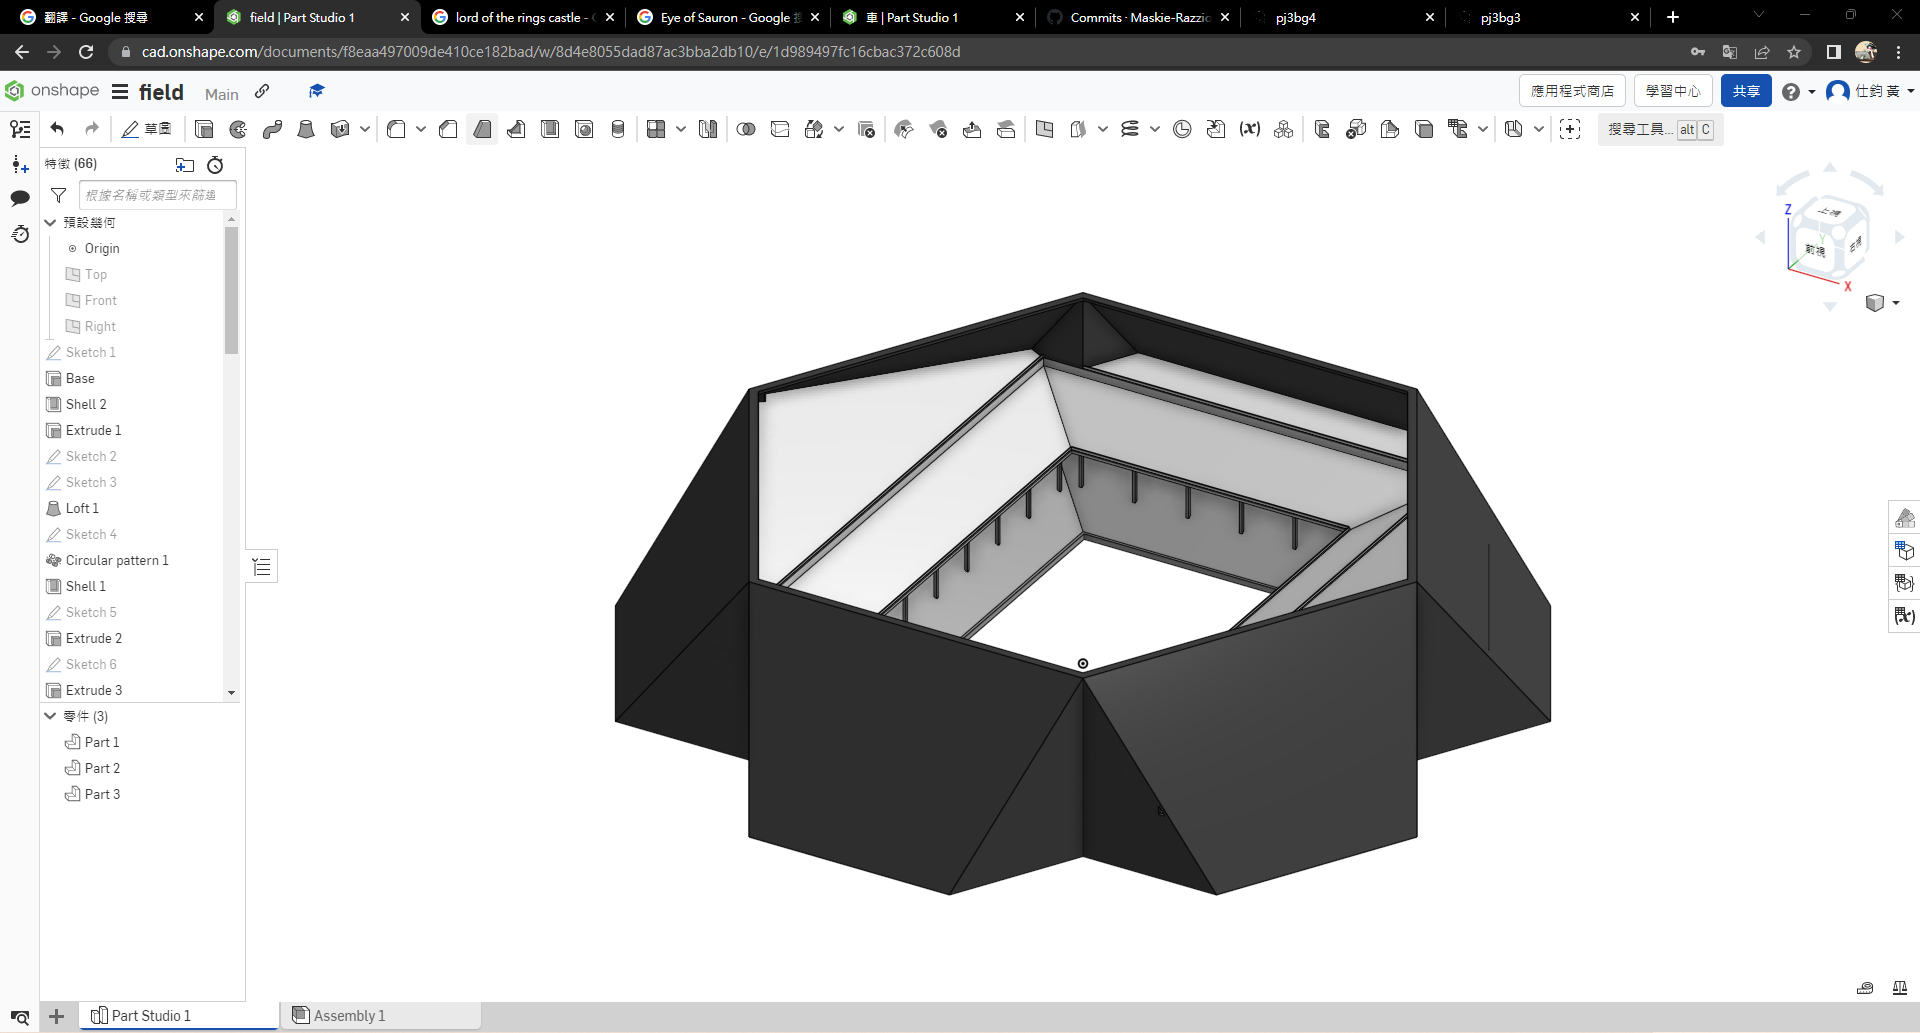
\includegraphics[width=0.5\textwidth]{field.png}
  \caption{球場圖片1}
  \label{fig:example}
\end{figure}


\begin{figure}
  \centering
  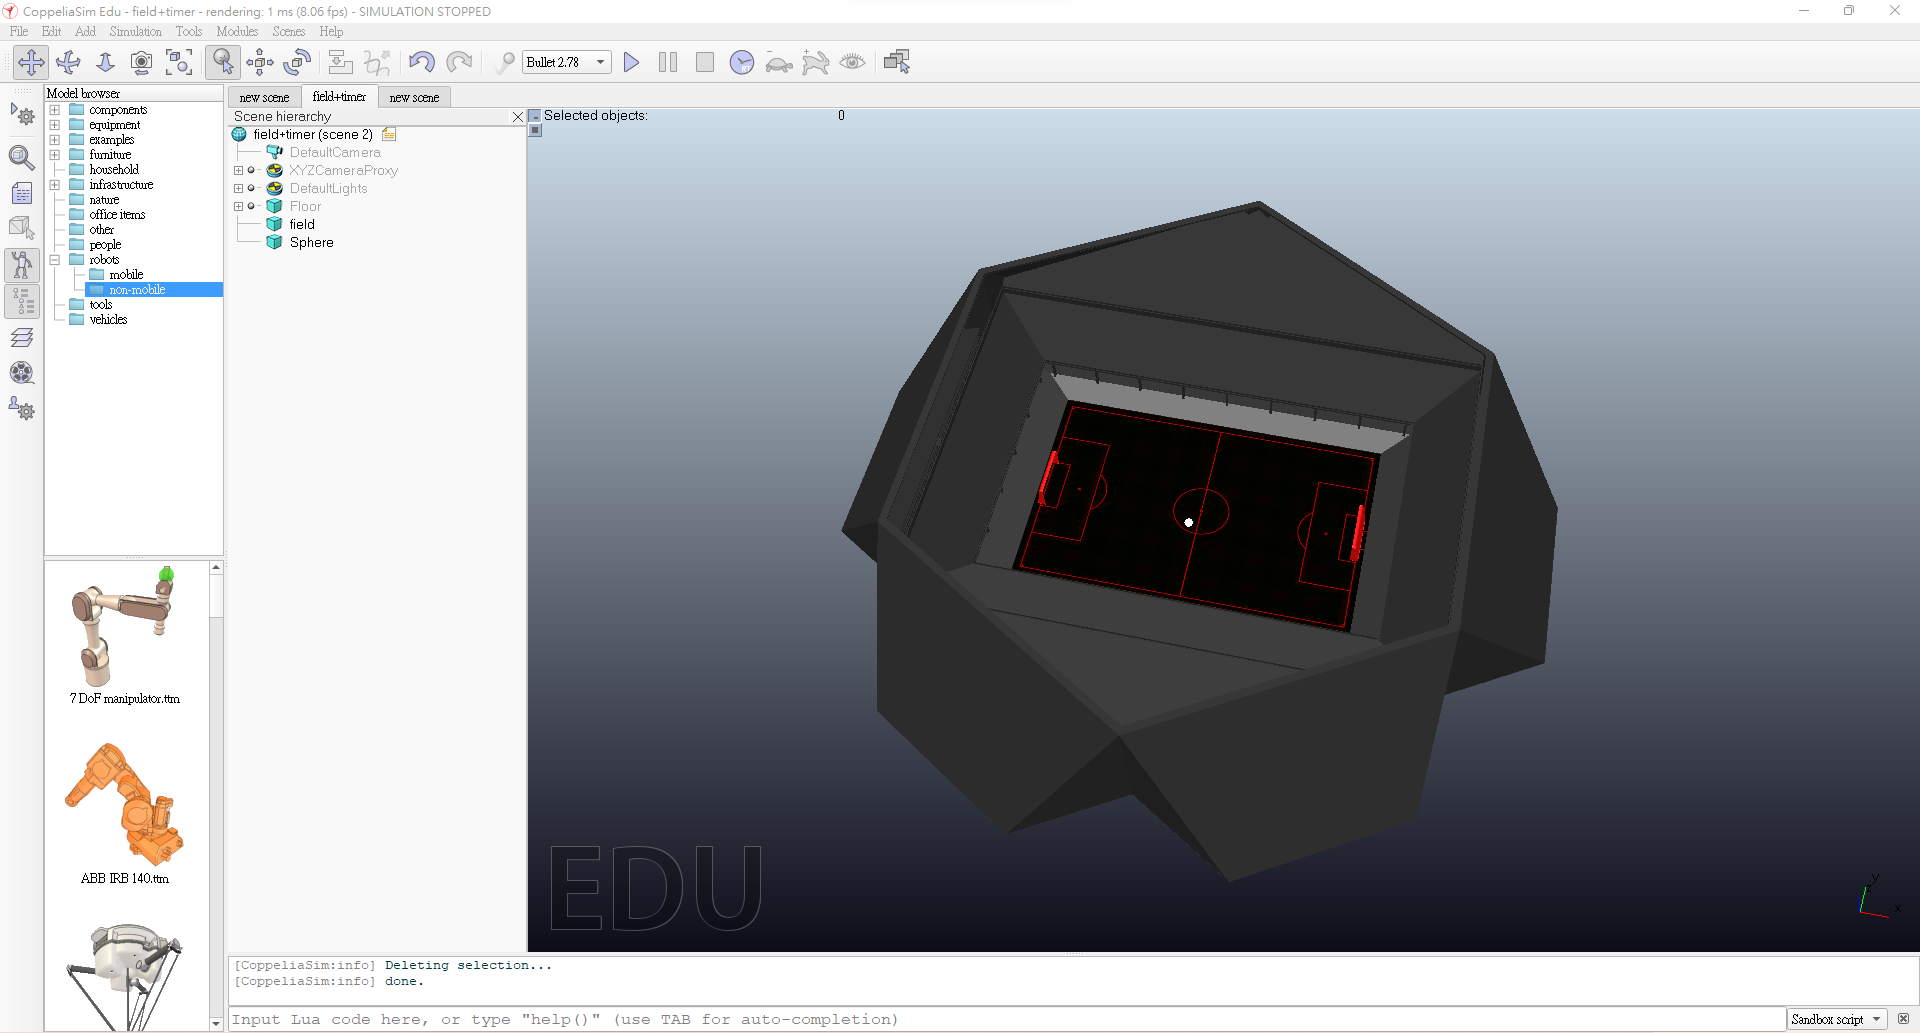
\includegraphics[width=0.5\textwidth]{field3.png}
  \caption{球場圖片2}
  \label{fig:example}
\end{figure}


\begin{figure}
  \centering
  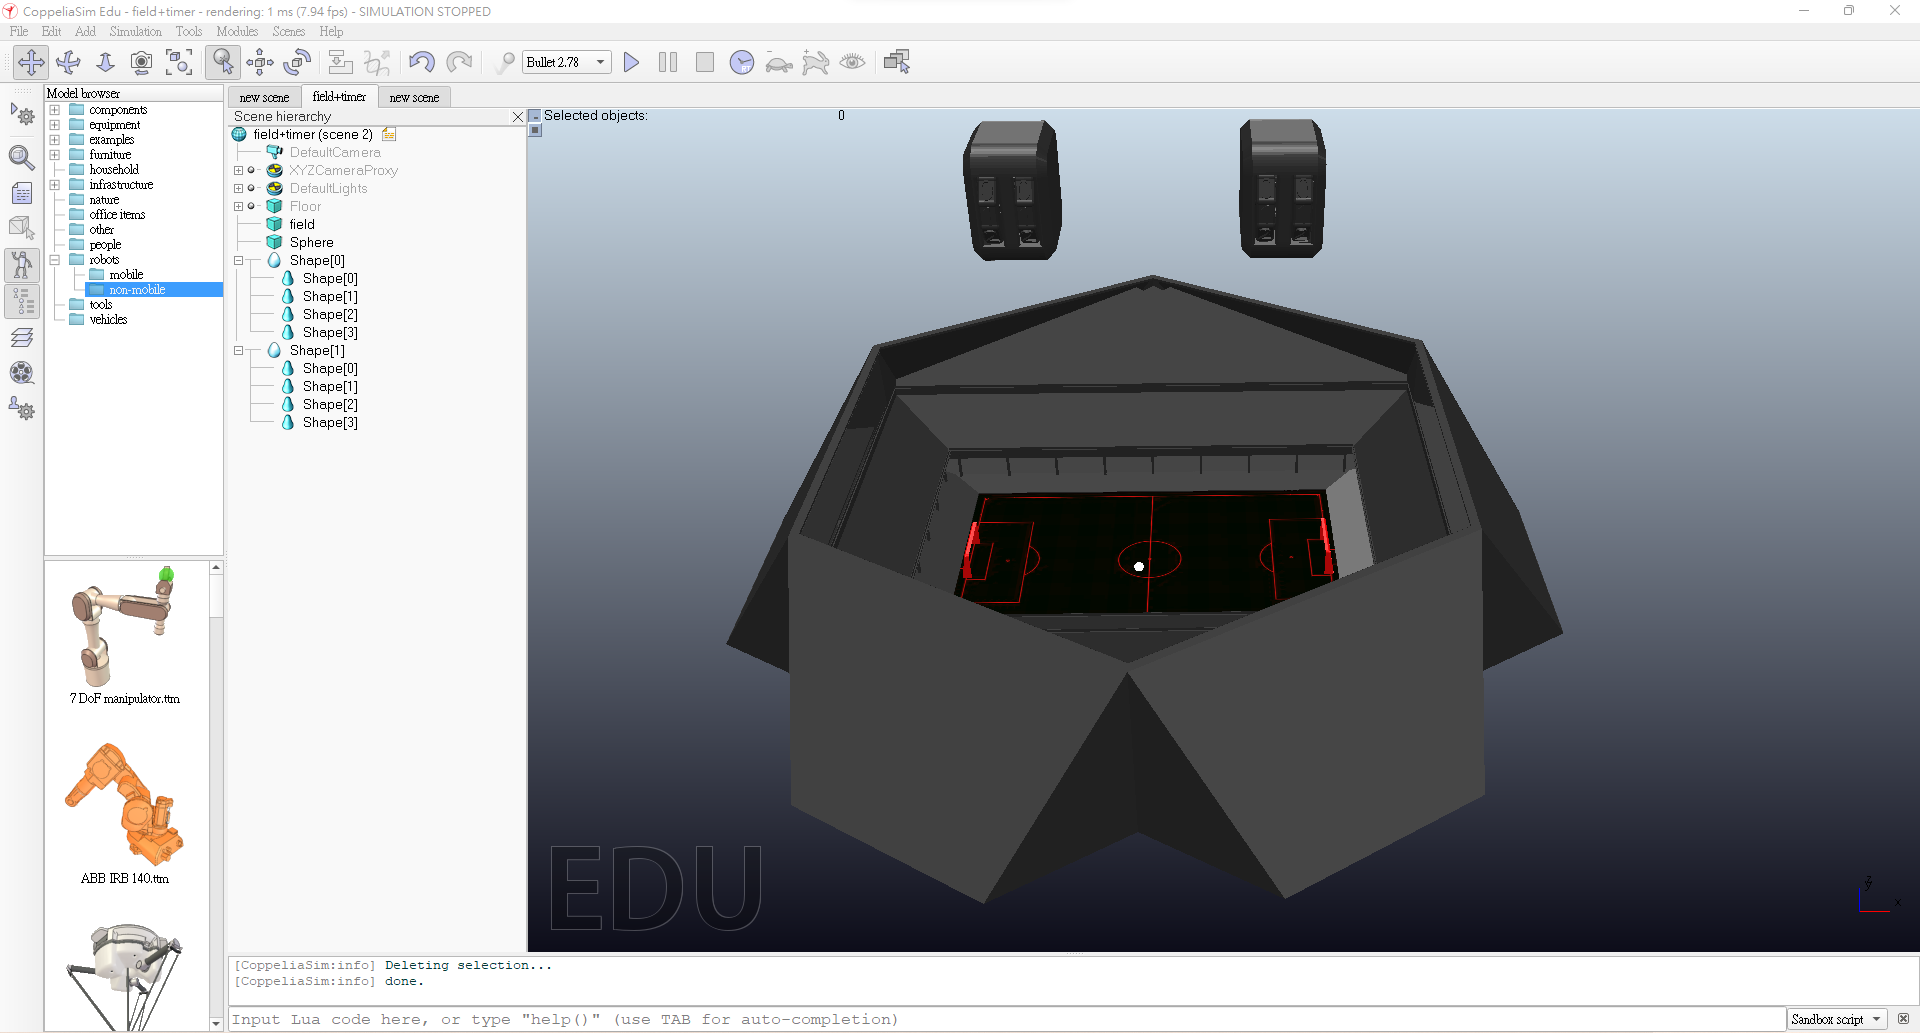
\includegraphics[width=0.5\textwidth]{CS-field2.png}
  \caption{球場圖片3}
  \label{fig:example}
\end{figure}


\begin{figure}
  \centering
  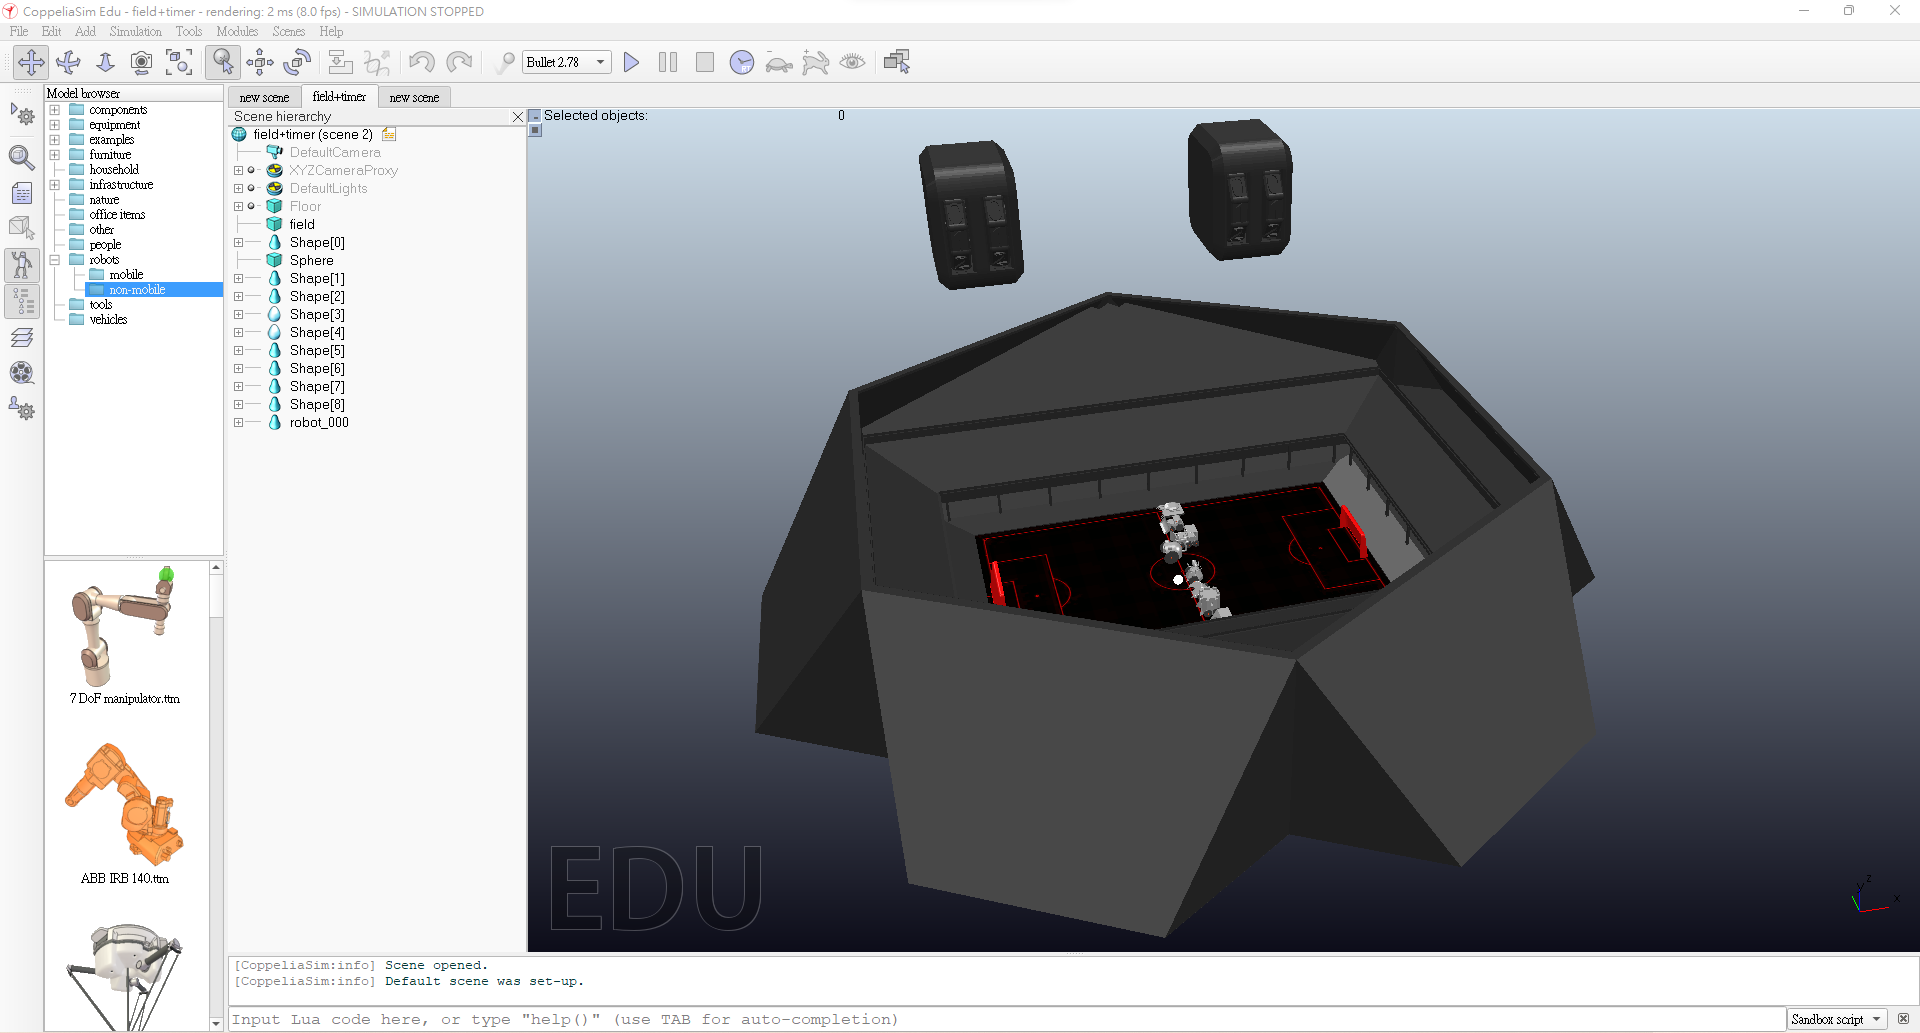
\includegraphics[width=0.5\textwidth]{CS-field.png}
  \caption{球場圖片4}
  \label{fig:example}
\end{figure}
\section{球員}